% Options for packages loaded elsewhere
\PassOptionsToPackage{unicode}{hyperref}
\PassOptionsToPackage{hyphens}{url}
\PassOptionsToPackage{dvipsnames,svgnames,x11names}{xcolor}
%
\documentclass[
  12pt,
  authoryear,
  preprint,
  3p]{elsarticle}

\usepackage{amsmath,amssymb}
\usepackage{lmodern}
\usepackage{iftex}
\ifPDFTeX
  \usepackage[T1]{fontenc}
  \usepackage[utf8]{inputenc}
  \usepackage{textcomp} % provide euro and other symbols
\else % if luatex or xetex
  \usepackage{unicode-math}
  \defaultfontfeatures{Scale=MatchLowercase}
  \defaultfontfeatures[\rmfamily]{Ligatures=TeX,Scale=1}
\fi
% Use upquote if available, for straight quotes in verbatim environments
\IfFileExists{upquote.sty}{\usepackage{upquote}}{}
\IfFileExists{microtype.sty}{% use microtype if available
  \usepackage[]{microtype}
  \UseMicrotypeSet[protrusion]{basicmath} % disable protrusion for tt fonts
}{}
\makeatletter
\@ifundefined{KOMAClassName}{% if non-KOMA class
  \IfFileExists{parskip.sty}{%
    \usepackage{parskip}
  }{% else
    \setlength{\parindent}{0pt}
    \setlength{\parskip}{6pt plus 2pt minus 1pt}}
}{% if KOMA class
  \KOMAoptions{parskip=half}}
\makeatother
\usepackage{xcolor}
\setlength{\emergencystretch}{3em} % prevent overfull lines
\setcounter{secnumdepth}{5}
% Make \paragraph and \subparagraph free-standing
\ifx\paragraph\undefined\else
  \let\oldparagraph\paragraph
  \renewcommand{\paragraph}[1]{\oldparagraph{#1}\mbox{}}
\fi
\ifx\subparagraph\undefined\else
  \let\oldsubparagraph\subparagraph
  \renewcommand{\subparagraph}[1]{\oldsubparagraph{#1}\mbox{}}
\fi


\providecommand{\tightlist}{%
  \setlength{\itemsep}{0pt}\setlength{\parskip}{0pt}}\usepackage{longtable,booktabs,array}
\usepackage{calc} % for calculating minipage widths
% Correct order of tables after \paragraph or \subparagraph
\usepackage{etoolbox}
\makeatletter
\patchcmd\longtable{\par}{\if@noskipsec\mbox{}\fi\par}{}{}
\makeatother
% Allow footnotes in longtable head/foot
\IfFileExists{footnotehyper.sty}{\usepackage{footnotehyper}}{\usepackage{footnote}}
\makesavenoteenv{longtable}
\usepackage{graphicx}
\makeatletter
\def\maxwidth{\ifdim\Gin@nat@width>\linewidth\linewidth\else\Gin@nat@width\fi}
\def\maxheight{\ifdim\Gin@nat@height>\textheight\textheight\else\Gin@nat@height\fi}
\makeatother
% Scale images if necessary, so that they will not overflow the page
% margins by default, and it is still possible to overwrite the defaults
% using explicit options in \includegraphics[width, height, ...]{}
\setkeys{Gin}{width=\maxwidth,height=\maxheight,keepaspectratio}
% Set default figure placement to htbp
\makeatletter
\def\fps@figure{htbp}
\makeatother

\usepackage{booktabs}
\usepackage{longtable}
\usepackage{array}
\usepackage{multirow}
\usepackage{wrapfig}
\usepackage{float}
\usepackage{colortbl}
\usepackage{pdflscape}
\usepackage{tabu}
\usepackage{threeparttable}
\usepackage{threeparttablex}
\usepackage[normalem]{ulem}
\usepackage{makecell}
\usepackage{xcolor}
\usepackage{placeins}
\usepackage{setspace}
\usepackage{lineno}
\onehalfspacing
\linespread{2}
\linenumbers
\makeatletter
\makeatother
\makeatletter
\makeatother
\makeatletter
\@ifpackageloaded{caption}{}{\usepackage{caption}}
\AtBeginDocument{%
\ifdefined\contentsname
  \renewcommand*\contentsname{Table of contents}
\else
  \newcommand\contentsname{Table of contents}
\fi
\ifdefined\listfigurename
  \renewcommand*\listfigurename{List of Figures}
\else
  \newcommand\listfigurename{List of Figures}
\fi
\ifdefined\listtablename
  \renewcommand*\listtablename{List of Tables}
\else
  \newcommand\listtablename{List of Tables}
\fi
\ifdefined\figurename
  \renewcommand*\figurename{Figure}
\else
  \newcommand\figurename{Figure}
\fi
\ifdefined\tablename
  \renewcommand*\tablename{Table}
\else
  \newcommand\tablename{Table}
\fi
}
\@ifpackageloaded{float}{}{\usepackage{float}}
\floatstyle{ruled}
\@ifundefined{c@chapter}{\newfloat{codelisting}{h}{lop}}{\newfloat{codelisting}{h}{lop}[chapter]}
\floatname{codelisting}{Listing}
\newcommand*\listoflistings{\listof{codelisting}{List of Listings}}
\makeatother
\makeatletter
\@ifpackageloaded{caption}{}{\usepackage{caption}}
\@ifpackageloaded{subcaption}{}{\usepackage{subcaption}}
\makeatother
\makeatletter
\@ifpackageloaded{tcolorbox}{}{\usepackage[many]{tcolorbox}}
\makeatother
\makeatletter
\@ifundefined{shadecolor}{\definecolor{shadecolor}{rgb}{.97, .97, .97}}
\makeatother
\makeatletter
\makeatother
\journal{Fisheries Research}
\ifLuaTeX
  \usepackage{selnolig}  % disable illegal ligatures
\fi
\usepackage[]{natbib}
\bibliographystyle{elsarticle-harv}
\IfFileExists{bookmark.sty}{\usepackage{bookmark}}{\usepackage{hyperref}}
\IfFileExists{xurl.sty}{\usepackage{xurl}}{} % add URL line breaks if available
\urlstyle{same} % disable monospaced font for URLs
\hypersetup{
  pdftitle={Methods to utilize known habitat to filter data for indices of abundance from a recreational fishery survey in California},
  pdfauthor={Melissa Hedges Monk; Rebecca R. Miller; Grant Waltz; Dean Wendt},
  pdfkeywords={fisheries dependent data, habitat
association, groundfish, index of abundance},
  colorlinks=true,
  linkcolor={blue},
  filecolor={Maroon},
  citecolor={Blue},
  urlcolor={Blue},
  pdfcreator={LaTeX via pandoc}}

\setlength{\parindent}{6pt}
\begin{document}

\begin{frontmatter}
\title{Methods to utilize known habitat to filter data for indices of
abundance from a recreational fishery survey in California}
\author[1]{Melissa Hedges Monk%
\corref{cor1}%
\fnref{fn1}}
 \ead{melissa.monk@noaa.gov} 
\author[2]{Rebecca R. Miller%
%
}
 \ead{rebecca.miller@noaa.gov} 
\author[33]{Grant Waltz%
%
}
 \ead{cat@example.com} 
\author[3]{Dean Wendt%
%
}
 \ead{cat@example.com} 

\affiliation[1]{organization={Southwest Fisheries Science
Center}, addressline={110 McAllister Way}, city={Santa
Cruz}, country={}, postcode={95060}}

\affiliation[2]{organization={University of California Santa
Cruz}, addressline={Street Address}, city={Santa
Cruz}, country={}, postcode={95060}}

\affiliation[3]{organization={California Polytechnic State
University}, addressline={Street Address}, city={San Luis
Obispo}, country={}, postcode={93407}}


\cortext[cor1]{Corresponding author}
\fntext[fn1]{This is the first author footnote.}



        
\begin{abstract}
Indices of abundance developed from fishery-dependent data are typically
subject to a number of assumptions about the area and habitat fished due
to the aggreation of the catch at the level of a fishing trip. In
California, two surveys occur onboard the recreational charter boats
fleet and samplers record location-specific data on the catch and effort
during individual fishing stops throughout a trip. This location
specific information coupled with high-resolution maps of the bottom
substrate allowed us to subset the the survey data to areas of rocky
reef habitat. The six species of rockfish (\emph{Sebastes} spp.) modeled
in this paper as example all have high affinity to rocky habitat. We
compared the indices of abundance developed from data filtering at the
finest scale of a fishing drop using the maps of rocky reef to filter
the data to the same data using only county of landing as an indicator
of location. In addition, we aggregated the data across a trip to mimic
data available from a dockside survey that occurs after a fishing trip
to further explore the effect of datacourseness on data filtering an
indices of abundance. For the data without any fishing location
identified we applied the commonly used Stephens-MacCall method to
identfy samples for the indices of abundance. The identification of the
rocky reefs also allowed us to weight the index of abundance by the area
of available habitat with predefined regions. We show that in general
the
\end{abstract}





\begin{keyword}
    fisheries dependent data \sep habitat
association \sep groundfish \sep 
    index of abundance
\end{keyword}
\end{frontmatter}\ifdefined\Shaded\renewenvironment{Shaded}{\begin{tcolorbox}[borderline west={3pt}{0pt}{shadecolor}, interior hidden, breakable, enhanced, boxrule=0pt, sharp corners, frame hidden]}{\end{tcolorbox}}\fi

\hypertarget{introduction}{%
\section{Introduction}\label{introduction}}

Integrated fisheries stock assessment models utilize a variety of data
sources to develop the most complete picture of the stock and current
status. Indices of abundance are one such data stream that provide a
time series of an observed portion of the stock with the assumption that
the trends are proportional to the stock's abundance
\citep{Harley:2001:CUE}. Ideally, a stock assessment would incorporate
indices of abundance developed from both fishery-independent surveys and
fishery-dependent surveys. It can often be the case that only
fishery-dependent data are available due factors including the lower
cost to collect fishery-dependent data, increased opportunities data
collection and the ease of which data can be collected. For
fishery-dependent data, catch per unit effort (CPUE) is a common metric
that provides information on the relative density of fish encountered
\citep{Maunder:2004:SCE}. more on F-D data

Within the recreational CPFV fleet, the target species can change within
a trip and between trips is are dependent on a number of factors. Some
of these factors include weather that could limit transit to some
fishing grounds, bag limit regulations, angler preference and
experience, and the captain's experience level. In order to create an
index of abundance from fishery-dependent data an analyst must be able
to subset the fishery-dependent data to those samples that fished in the
appropriate location for a species of interest.

Depending on the target species, the data may contain a high proportion
of zero observations across samples. The question arises as to whether
fishing occurred within the species of interest's habitat and the
species was not observed or if the sampling occurred outside of the
species' habitat (structural zeroes). Including structural zeroes in the
models used to standardize of indices of abundance adds noise and added
variability (citation). Fishery surveys of the recreational CPFV fleet
often occur after fishing for the day has ended. These data often report
a single fishing location for a trip, but it is often the case that
multiple locations are fished over the course of the day and may or may
not encounter the same suite of species depending on factors such as
depth, bottom habitat type, and other environmental conditions.

Here we focus on data available from a fishery-dependent survey of the
recreational partyboat (commercial passenger fishing vessel fleet
(CPFV)) in California, specifically a survey where a sample rides along
on paid fishing trips (onboard observer survey). The effort on the
onboard observer survey is the number of anglers multiplied by the
amount of time fished, to produce angler hours. In addition, we are able
to utilize high resolution bathymetric data to define appropriate
habitat for the target rockfish (\emph{Sebastes} spp.) species.

It is not often the case where high-resolution habitat data and fishing
location information are both available, and for many fishery-dependent
surveys an analyst will have to determine which subset of the data to
use based on available information. The onboard observer data provide an
opportunity to explore what information we gain from explicit knowledge
of fishing locations. There are two surveys of the California
recreational CPFV fleet, both using the same methodologies, that provide
information on the catch, effort and fishing location during CPFV trips
\citep{Monk:2014:DRD}. Both the California Department of Fish and
Wildlife (CDFW) and the California Polytechnic State University San Luis
Obispo (Cal Poly) conduct a survey where a sampler rides along during a
CPFV trip with paid anglers and records data at each individual fishing
stop (referred to as the onboard observer surveys). Paired with recently
available high-resolution bathymetry data provided an opportunity to map
each individual fishing drift onto known habitat type (hard vs.~soft
substrate).

One of the major recreational targets in California are bottomfish
species, a group of over 100 species, 92 of which are rockfish species
(\emph{Sebastes spp.}). Many of the recreationally targeted rockfish
have a high association to rocky habitat as adults. The affinity to
rocky habitat differs by species and ranges from a species like the
gopher rockfish (\emph{Sebastes carnatus}) that resides within crevices,
to schooling species that inhabit the mid-water such as the black
rockfish (\emph{Sebastes melanops}). The association of these species
make them ideal candidates for exploring the ability to filter
fishery-dependent data based on known habitat. In addition, the habitat
data creates an opportunity to weight the index of abundance by the
calculated area of rocky reef habitat along the California coast. xxxxxx

To explore how indices of abundance change depending on assumptions made
during the data filtering steps, we utilized the onboard observer data
create data sets and indices at three levels of data courseness. At the
finest scale we utilized the fishing drift level data with known
location from the onboard observer surveys and subset data based on the
proximity to rocky reef habitat. We then treated the drift-level data as
if the location of the individual fishing drifts were not available, and
lastly, we aggregated the drift-level catches to the level of a single
trip. For the last two two cases where we removed the location
information, we filtered the data using the Stephens-MacCall method. We
applied these methods across six nearshore rockfish species with
different life histories,habitat preferences and commonness in the data.

A commonly used method to filter fishery-dependent data to the samples
representing the effect fishing effort of the target species and exclude
structural zeroes is the Stephens-MacCall method
\citeyearpar{Stephens:2004:MAS}. The Stephens-MacCall method is a
binomial model used to predict the probability of encountering the
target species in a sample, based on the presence and absence of a suite
of co-occurring species. This method is commonly used to filter data
that are collected dockside after a vessel returned to port or when
location data are not provided. We applied the Stephen-MacCall method to
both the trip-level data and the drift-level data to explore differences
in the courseness of species composition effects data filtering and the
index of abundance.

\hypertarget{methods}{%
\section{Methods}\label{methods}}

We developed indices of abundance for six species or species pairs of
rockfish (\emph{Sebastes spp.}) that are of management interest on the
U.S. West Coast: black rockfish (\emph{S. melanops}), the blue and
deacon rockfish (\emph{S. mystinus}/\emph{S. diaconus}), brown rockfish
(\emph{S. auriculatus}), China rockfish (\emph{S. nebulosus}), gopher
rockfish (\emph{S. carnatus}), and the vermilion and sunset rockfish
(\emph{S.miniatus}/\emph{S. crocotulus}). The two cryptic species pairs
(blue/deacon and sunset/vermilion rockfish) are genetically
identifiable, but not separable within the onboard observer survey time
series. These six species all have different latitudinal distributions,
exploitation histories, and habitat and depth
preferences\citep{Love:2002:RNP}.

\hypertarget{survey-data-and-habitat-based-filtering}{%
\subsection{Survey Data and Habitat-based
Filtering}\label{survey-data-and-habitat-based-filtering}}

The California Department of Fish and Wildlife (CDFW) began a
fishery-dependent onboard observer survey of the Commercial Passenger
Fishing Vessel (CPFV or party/charter boat) fleet in 1999. In 2004, the
survey became part of the CDFW's California Recreational Fisheries
Survey (CFRS, \emph{add year and cite website}) that includes additional
surveys to quantify catch and effort by the recreational fleet. In
response to a request from the fishing industry, the California
Polytechnic State University Institute of Marine Science, San Luis
Obispo (Cal Poly) began a supplemental onboard observer survey in 2001
of the CPFV fleet based in Port Avila and Port San Luis along the
Central Coast {[}\#fig-map{]}. Both the CDFW and the Cal Poly onboard
observer surveys continue through present day; however, due to both
spatial and temporal recreational regulation changes we limited the data
for this research to the years 2004 to 2016. Between 1999 and 2003, the
recreational regulations evolved from no restriction on the number of
lines or hooks an angler could deploy to a one line and two-hook
maximum, as well as implementation of depth restrictions. Subsequent
management allowed a relaxation of depth restrictions beginning in 2017,
potentially shifting fishing effort relative to the 2004-2016 period
\citep{Monk:2021:SVR}.

While only a small portion of the total CPFV trips taken are sampled as
part of the onboard observer survey, the onboard observer survey
collects a large amount of data during each trip. During each trip the
sampler records information for each fishing drift, defined as a period
starting when the captain announced ``lines down'' to when the captain
instructs anglers to reel their lines up. Just prior to the start of
each fishing drift, the sampler selected a subset of anglers to observe,
at a maximum of 15 anglers per drift. The sampler records all fish
encountered (retained and discarded) by the subset of anglers as a
group, i.e., catch cannot be attributed to an individual angler.
Samplers also record the start and end times of a drift, location of the
fishing drift (start latitude/longitude and for most drifts, end
latitude/longitude), and minimum and maximum bottom depth. Fish
encountered by the group of observed anglers are recorded as either
retained or discarded. This provides information on the catch (count of
each species) and effort (time and number of anglers fished) during each
fishing drift. While both surveys include records of discarded fish, we
only used the retained catch in these analyses. Discarded fish can often
represent a different size structure than retained fish, either due to
size limits or angler preference, or represent fish encountered during a
temporal or spatial closure.

The SWFSC developed a relational database for the CDFW onboard survey
from 1999-2010\citeyearpar{Monk:2014:DRD} that has been updated
annually. The Cal Poly data are also provided to the SWFSC annually. All
data were checked for potential errors at the drift-level by SWFSC
staff.

The CPFV data included only areas north of Point Conception
(\(34^\circ 27^\prime N\)) due to gaps in habitat coverage further
south. Point Conception is a significant biogeographic boundary
(\citet{Newman:1976:HBP}), the composition of the fish communities in
southern California differ, and the recreational fisheries are
fundamentally different, with a higher percentage of trips targeting
mixed species and pelagic and highly migratory species, as well as more
limited access to rocky habitat nearshore.

After filtering the data to north of Point Conception, we further
removed drifts that may not accurately define a successful fishing drift
or represent data errors, the upper and lower 1\% of the recorded time
fished and recorded observed anglers were removed. Given that the
fishery was closed deeper than 40 fathoms for the entire time period
from 2004-2016, we filtered the data to retain 99\% of all drifts based
on average drift depth. We calculated average depth from the recorded
minimum and maximum depths when available or the imputed minimum and
maximum depth from the bathymetry layer described in the next paragraph.
A depth cutoff slightly deeper than the maximum allowed is reasonable
given the variability in habitat fished and all retained drifts occurred
within California state waters (up to 3 nm from shore).

High resolution seafloor mapping data allowed us to map each drift from
the onboard observer surveys with predicted habitat (referred throughout
the paper as the drift-level, habitat-informed data). We utilized the
bathymetry and backscatter data collected by the California Seafloor
Mapping Program (CSMP) \citep{Golden:2013:CSW}. The CSMP mapped
California state waters at a 2 m resolution north of of Point Conception
to the California-Oregon border. A total of 137 CSMP substrate blocks
that ranged in size from 16 \(km^2\) to more than 400 \(km^2\) were
mosaicked together by authors. Rough and smooth substrates were
identified by CSMP using two rugosity indices, surface:planar area, and
vector ruggedness measure (VRM) of the bathymetric digital elevation
model {[}\#fig-map2{]}. The CSMP set a varying VRM threshold for each of
the substrate blocks, removed any artifacts, and is considered a
conservative estimate of rough habitat.

The 137 CSMP substrate raster blocks were then mosaicked together by
authors, and converted the pixels designated as rough habitat (rocky
habitat proxy) from a raster format to polygons, and calculated a 5 m
buffer around the rough habitat polygon to allow for any small errors in
positional accuracy using ArcMap 10.7 (ESRI citation). The area of each
reef polygon was calculated, and those reefs greater than or equal to
100 \(m^2\) were included. Contiguous polygons identified as rocky
substrate were defined as a singular rocky reef, regardless of size. The
area of rocky habitat for this paper was calculated to exclude portions
of the reef that extended outside of California state waters (further
than 3 nm from shore). The mapped area does not include very shallow
areas close to shore, which extend approximately 200-500 m from the
shoreline. Fishing by the CPFV fleet is limited in these waters due to
shallow depths and kelp beds. We assigned fishing drifts to reefs based
on the recorded start location of a drift, given that the end locations
of drifts were not always recorded. The distance from the recorded drift
start location to the nearest rocky habitat was calculated in meters.
For each target species, we calculated the cumulative distribution of
distance to rocky reef for drifts that retained the target species and
used a distance cutoff of 90\% for each species. To illustrate the
similarities and differences among the six species, we plotted the
percent of fishing drifts within an aggregated region that where the
species was present and retained. To show the differences in the general
commonness or rarity of the species we calculated the average CPUE,
before standardization, for each species and aggregated area. We also
downloaded the effort estimates for the CPFV trips from RecFIN to
compare the the the area of rocky habitat with the effort in each region
as well as the distribution of observed trips.

\hypertarget{stephens-maccall-data-filtering}{%
\subsection{Stephens-MacCall Data
Filtering}\label{stephens-maccall-data-filtering}}

We applied the Stephens-MacCall method to both the drift-level data and
the trip-level data \citeyearpar{Stephens:2004:MAS}. For the drift-level
data we removed all location and depth identifiers for a drift and kept
the county of landing as a spatial identifier. To construct a data set
that mimicked trip-level data, we took the drift-level data, aggregated
the observed retained catch within a trip, and kept the county of
landing as a spatial identifier. We then compared results using two
levels of aggregation (catch rates by drift and trip) to illustrate the
impact of having less spatially-explicit data on both data filtering and
the resulting indices of abundance.

Prior to any filtering a total of 19,425 drifts that aggregated to 2,270
trips were available for the analyses. The number of initial samples
used for the Stephens-MacCall filtering method were higher than the
habitat-informed data described in the previous section because retained
drifts with missing locations (latitude/longitude).

Before applying the Stephens-MacCall method, we identified a suite of
potentially informative predictor species for each of the six target
species. Species that never co-occurred with the target species and
those present in fewer than 1\% of all drifts and 3\% of all trips were
removed to reduce the number of species to those that were informative.
A lower threshold of 1\% was selected for the drift-level data due to
the change in magnitude of the number of samples when using drifts vs
trips.

The remaining species all co-occurred with the target species in at
least one trip and were retained for the Stephens-MacCall logistic
regression. Coefficients from the Stephens-MacCall analysis (a binomial
generalized linear model) were positive for species that are more likely
to co-occur with the target species, and negative for species that were
less likely to be caught with target species. The intercept represented
the probability of observing only the target species in a sample. We
also calculated the 95\% confidence interval for each coefficient.

Stephens and MacCall proposed filtering (excluding) samples from index
standardization based on a criterion of balancing the number of false
positives and false negatives from the predicted probability of
encounter. False positives (FP) are trips that are predicted to
encounter the target species based on the species composition of the
catch, but did not. False negatives (FN) are trips that were not
predicted to encounter the target species, given the catch composition,
but caught at least one target species. Stephens and MacCall recommended
a threshold where the false negatives and false positives are equally
balanced, however, this threshold does not have any biological relevance
and for this particular data set where trained samplers identify all
fish. We assumed that if the target species was encountered, the vessel
fished in appropriate habitat.

Of interest for the index of abundance was the elimination of trips that
had a low probability of catching the target species given the other
species caught on the trip. Therefore, we retained all of the trips that
caught the target species and those trips that did not catch the target
species, but had a probability higher than the threshold balancing the
false negatives and false positives. This practice has commonly been
used in recent stock assessments of rockfish on the West Coast.

\hypertarget{indices-of-abundance}{%
\subsection{Indices of Abundance}\label{indices-of-abundance}}

Four standardized indices of abundance were generated for each of the
six species, one each for the data filtering method (drift-level
habitat-informed, drift-level Stephens-MacCall, trip-level
Stephens-MacCall) and an area-weighted index from the habitat-informed
drift-level data. All indices were modeled using Bayesian generalized
linear models (GLMs) and the delta GLM method
\citep{Lo:1992:IRA, Stefansson:1996:AGS}. The delta GLM method is
commonly used to standardize catch-per-unit effort for stock assessments
{[}citations{]}. The delta method models the the data with two separate
GLMs; one for the probability of encountering the species of interest
from a binomial likelihood and a logit link function and the second
models the positive encounters with either gamma or lognormal error
structure. The error structure of the positive model was selected via
the Akaike Information Criterion (AIC) from models with the full suite
of considered explanatory variables.

The response variable for the positive models was angler-retained catch
per unit effort. For the indices modeled at the level of a drift, effort
was calculated as the number of angler hours fished on a drift. The
trip-level effort was calculated as angler days, using the average
number of observed anglers across all drifts on a trip.

To keep comparisons across data filtering methods similar, depth was not
considered as an explanatory variable in the habitat-informed index.
Depth is often a significant explanatory variable for rockfish species,
with many rockfish species and populations separated by depth
\citep{Love:2002:RNP}. Year was always included in as an explanatory
variable in model selection, even if it was not significant, because the
goal of the index of abundance was to extract the year effect. Other
explanatory variables considered for the habitat-informed index were
aggregated regions rocky reefs (categorical variable\emph{)} and wave (a
3-month aggregated period of time, e.g., January-March). The
area-weighted index also included a year/rocky reef interaction term,
even if it was not statistically significant, to allow us to weight the
index by the area of rocky reef. The regions of rocky reef were
aggregated differently for each species to ensure adequate sample sizes
to explore the year/rocky reef interaction.

Explanatory variables for the two indices using the data filtered using
Stephens-MacCall method (blind to habitat information at the drift- and
trip-level) included only year, wave and aggregated counties of landing.
California has 14 coastal counties north of Point Conception, 11 of
which were represented in these data. We aggregated the northern
counties of Del Norte, Humboldt and Mendocino into one region, Sonoma
and Marin counties just north of San Francisco into another region and
Alameda and San Francisco counties into a third region. The remaining
counties of San Mateo, Santa Cruz, Monterey and San Luis Obispo remained
unaggregated.

Model selection for the binomial and positive observation models was
based on AIC using the lme4 package in R, and unless very different
predictors were selected, the same predictors were used in each of the
two Bayesian models. The Bayesian models were run with 5,000 iterations
and weakly informative priors. Posterior predictive model checks were
examined for both the binomial and positive observation models,
including the predicted percent positive compared to the maximum
likelihood estimates. We constructed the final year index by multiplying
the back-transformed posterior draws from the binomial model with the
exponentiation of positive model draws, and taking the mean and standard
deviation for each year.

The area-weighted habitat-informed index was developed by extracting the
posterior draws of from each year and area combination of the binomial
and positive posterior predictions, and then summing across the product
of the back-transformed posteriors weighted by the fraction of total
area within each reef. To compare the indices across the three data
filtering methods and the area-weighted index, each index was scaled to
its mean value.

\hypertarget{results}{%
\section{Results}\label{results}}

\hypertarget{survey-data-and-habitat-based-filtering-1}{%
\subsection{Survey Data and Habitat-based
Filtering}\label{survey-data-and-habitat-based-filtering-1}}

The data sets were filtered for errors within the relational database
before analyses were conducted, and the data used here reflect changes
from the QA/QC process that may not be reflected in the raw data
available directly from the CDFW. Approximately 21\% of all the CDFW
observed CPFV trips from 2004-2016 occurred north of Point Conception
and it is important to note that north of Bodega Bay, California, the
majority of charter boats are smaller 6-pack vessel that may not have
the capacity to carry a sampler onboard. The addition of the Cal Poly
onboard observer survey to the CDFW survey increased the sample sizes of
observed trips in San Luis Obispo county by an average of 155\% from
2004-2016.

From 2004-2016 the drift-level data contained a total of 19,425 fishing
drifts, and after removing drifts with missing effort information (time
fished and/or observed anglers), 19,180 drifts remained. The filter
removing the upper and lower 1\% of the time fished and number of
observed anglers resulted in fishing drifts lasting between three and 96
minutes and three to 15 observed anglers, and reduced the data to 18,591
fishing drifts. The remaining data filter for depth resulted in a cutoff
of 46.6 fathoms, and retained 18,405 drifts based on average drift
depth. A filter on the minimum depth was not included here because the
recreational fleet was not limited to a minimum fishing depth and all of
the fishing drift locations were verified during the QA/QC process.

We defined 108 areas of rocky habitat within California state waters
from the California/Oregon border to Point Conception. The 2 m
resolution of the substrate shows the patchiness and heterogeneity of
the rocky substrate (Figure~\ref{fig-map2}). We adopted the same
thresholds to define rocky habitat as determined by the United States
Geological Survey (USGS). While the location-specific data from the
fishing fleet is governed by confidentiality and cannot be displayed
here, 85\% of the fishing drifts were withing 5 m of rocky habitat. The
recreational fishing fleet's targeting of rockfish species was verified
by the distributions of the distance from rocky habitat for each of the
six species. The distance from rocky habitat cutoff (retaining 90\% of
drifts encountering each species) for blue, China and gopher rockfish
was six meters, eight meters for vermilion rockfish, 14 meters for black
rockfish and 16 meters for brown rockfish. The percentage of drifts and
trips encountering the target species can be found in
Table~\ref{tbl-samplesize}.

Based on exploratory analyses and consideration of the available data,
the areas of rocky habitat were grouped into six regions to ensure
adequate sample sizes for developing indices of abundance
(Figure~\ref{fig-map}). While covering a small area (5\% of the rocky
habitat), the number of observed fishing drifts within state waters
around the Farallon Islands off the coast of San Francisco was high
enough to warrant keeping it as a separate area of rocky habitat. The
region defined from the California/Oregon to San Francisco encompasses
49\% of the total rocky habitat in state waters by area, but only 12\%
of the observed drifts (2,637) fished in this area. Each of the four
remaining regions of rocky habitat defined from San Francisco to Point
Conception contained an average of 12\% of the available habitat. The
CDFW estimated fishing effort by management district, which does not
exactly align with our areas of grouped reef habitat. Only considering
the fishing effort north of Point Conception, CDFW estimated an average
of 9\% of the CPFV from the California/Oregon border through Mendocino
County, 38\% from Sonoma through San Mateo County, and 53\% from Santa
Cruz to Point Conception.

The differences in latitudinal distribution of the six species is
apparent from the maps of percent of positive observations
(Figure~\ref{fig-percentpos}). Black rockfish are distributed north of
San Francisco, a more northerly distribution reflected in the
aggregation of data from Santa Cruz and south, whereas brown rockfish is
distributed across coastal California. Percent positive catch generally
showed higher catches south of San Francisco for vermilion, gopher,
brown, and blue rockfish. The percentage of drifts retaining China
rockfish was low coastwide. The average CPUE was highest for blue
rockfish between San Francisco south to Big Sur (Figure~\ref{fig-cpue}).
The average CPUE for black rockfish average CPUE was higher in the
north, while gopher rockfish CPUE was generally consistent across the
coast, albeit slightly higher south of Big Sur. China rockfish CPUE
catch was typically low coastwide, with slightly higher catch rates in
the Farallon Island reefs.

The final aggregation of the reefs and total area within each region are
found in Table~\ref{tbl-reefareas} and reflect the distribution and
patterns in the visual representation of commonness in the data. The
fraction of drifts retained for the indices of abundance was high for
all six species (80\% or greater), indicating that many of drifts within
these data occurred near areas of rocky habitat.

\hypertarget{stephens-maccall-data-filtering-1}{%
\subsection{Stephens-MacCall Data
Filtering}\label{stephens-maccall-data-filtering-1}}

A total of 19,425 drifts that aggregated to 2,252 trips were used for
the trip-level Stephens-MacCall filtering. In general, the co-occurring
species used for the Stephens-MacCall method were similar for the
drift-level and the trip-level data. We present the coefficients and
95\% confidence intervals for the species coefficients for black
rockfish and brown rockfish at the trip-level in Figure~\ref{fig-sm}.
The plots for black rockfish and brown rockfish at the drift-level and
all plots for the remaining four species are available in the
supplemental materials. The confidence intervals were larger for the
trip-level data and the co-occurring species at the drift-level provide
a refined look at species that have positive coefficients. For black
rockfish, a noticeable difference is the intercept. At the trip-level
the intercept (probability of catching the target species, given that
none of the indicator species were caught) is uninformative and at the
drift-level the intercept is strongly negative. A higher fraction of the
co-occurring species are uninformative information about the target
species in our study (the 95\% confidence interval crosses zero) for the
trip-level data than the drift-level.

The percentage of samples retained for each data filtering method
differed by species, but followed the general trend that the lowest
percent of samples were retained from the Stephens-MacCall filtering at
the drift level, ranging from 12\% of samples retained for China
rockfish and 54\% for blue rockfish (Table~\ref{tbl-samplesize}). A much
higher percent of samples were retained both from the other two methods,
with an average of 83\% of drifts retained when habitat was included as
a filter. Data filtering for the trip-level indices that retained all
positive observations resulted in a high proportion of positive samples
(0.70 - 0.86) for all species.

To determine how consistent the Stephens-MacCall trip-level filter was
with the habitat-informed filter, we looked at the distance to reef from
all of the drifts contributing to trips that were used for the
trip-level index. This provides a proxy for how well the
Stephens-MacCall method infers habitat from species associations. Using
the same distance from reef cutoff by species as calculated from the
habitat-informed data, we calculated the percentage of drifts that were
further from a reef than would be expected, but used in the data to
develop the trip-level index. The percentage of drifts contributing to
the trips outside reef habitat was 11\% for black rockfish, 13\% for
blue rockfish, 10\% for brown rockfish, 12\% for China rockfish, 12\%
for gopher rockfish, and 11\% for vermilion rockfish.

\hypertarget{indices-of-abundance-1}{%
\subsection{Indices of Abundance}\label{indices-of-abundance-1}}

All but three of the 24 indices of relative abundance were modeled with
a lognormal distribution. The trip-level indices for black, blue and
gopher rockfish were modeled using a gamma distribution as selected by
AIC (AIC values available in the supplementary material). All of the
covariates (year, reef, and wave) were selected for both the binomial
and positive models for all species in the habitat-informed drift level
index. Gopher rockfish was the only case for the drift-level
habitat-informed index where different models the covariates year and
reef were select over year, reef and wave. However, the change in AIC
was one so we chose to maintain the model with year, reef and wave.

(LMK and I can put these in a table in the doc) The full model that
included the reef:year interaction was selected by AIC for all species
except for China rockfish. For China rockfish the positive binomial
model selected the interaction covariate, but the model without the
interaction was select for the positive lognormal model by an difference
in AIC of 22. However, in order to look at the effects of the
area-weighting on the index, we included the year:reef interaction in
the final model for China rockfish.

For both the drift-level and trip-level Stephens-MacCall filtered data,
year, county and wave were selected for black rockfish, blue rockfish,
gopher rockfish, and vermilion rockfish and the drift-level index for
brown rockfish. The model incorporate in year and county was selected
for the trip-level Stephens-MacCall filtered index for brown rockfish
and both Stephens-MacCall filtered indices for China rockfish.

In general, the larger increases and decreases in the indices were
similar among the four indices developed for each species
(Figure~\ref{fig-indices}). The generalized approach used in this paper
to create indices with comparable methods resulted in different results
for each species. The area-weighted indices are reflective of the total
available habitat and use all of the available high resolution habitat
and fishing drift data. However, differences among the four indices were
different for each species. The average CVs between the drift-level
area-weighted index and the drift-level habitat informed indices were
similar, as expected, since they both used the same data with the only
difference being the year:area interaction in the models
(\citet{tab-avgcv}). However, the average CV between drift-level
habitat-informed filtering and Stephens-MacCall filtering for the
drift-level data differed by species.

The area-weighting for black rockfish, a species distributed
predominantly north of Santa Cruz, California did have an effect on the
index for a number of years, most notably in 2013 where the
area-weighted estimate is lower than all three other
indices(Figure~\ref{fig-black-indices}). The effect of the
area-weighting is also apparent for black rockfish in 2005, 2007, and
2009.The average CV decreased from the trip-level index (0.671) to to
the area-weighted index (0.443) and was lowest overall for the
drift-level Stephens-MacCall index (0.364) which also modeled much
smaller data with a high proportion of positive catches of black
rockfish (\citet{tab-samplesize}).

Blue rockfish is ubiquitous across the study area and was one of the two
species for which the area-weighting at the six most disaggregated
regions. The area-weighted index differs from the other three in 2006
with an estimated higher relative abundance and in 2014 with an
estimated lower relative abundance. Even during the years from 2009 to
2012 when the estimated relative abundance was low for all of the
indices, there were differences among the four trends with the
drift-level habitat-informed index estimating the lowest relative
abundance.

All four indices for brown rockfish suggested differing trends, with
this species having the highest estimated error for both the trip-level
and drift-level Stephens-MacCall filtered data
(Figure~\ref{fig-brown-indices}). In ten of the years the area-weighted
index estimated a either the largest or smallest relative abundance
compared to the other indices. For brown rockfish the two
habitat-informed indices were more similar than the Stphens-MacCall
filtered data. The average CV for brown rockfish from the
Stephens-MacCall filtering was large (0.679) compared to the habitat
informed filtering (0.142).

China rockfish is the only species for which the trip-level
Stephens-MaCall filtered index had the lowest average coefficient of
variation that increased with the the habitat-informed filtering
(\citet{tab-avgcv}). Although the trends among the four indices was
similar, this is the only species for which the highest error was
consistly estimated for both habiat-informed drift-level indices
(Figure~\ref{fig-china-indices}). China rockfish is one of the less
common species observed in the data with the highest average CPUE from
catches the Farallon Islands, which is an overall small percentage of
the total habitat (\citet{tab-reefareas}).

The observed trends for gopher rockfish were similar among all indices
and the trip-level Stephens-MacCall index had the highest average CV
(0.626) compared to the average CVs of less than two from all of the
other drift-level indices. China rockfish is the only species for which
the trip-level index had the lowest average coefficient of variation,
which increased with the the habitat-informed filtering . For all other
species, the habitat-informed filtering resulted indices with a lower
average CV than the trip-level filtering.

The indices of relative abundance for vermilion rockfish were relatively
similar in trends across the time series and
(Figure~\ref{fig-vermilion-indices}). Vermilion rockfish is the second
species for which all six areas of rocky reef habitat remained
disaggregated in the models. For vermilion rockfish, while the trends
are similar among all four indices, the effect of area-weighting dampens
the increase modeled from the habitat-informed drift level data from
2004-2006, where the area-weighting downweighted the relative abundance
from the drift-level habitat informed index.

\FloatBarrier

\hypertarget{discussion}{%
\section{Discussion}\label{discussion}}

We demonstrated new methodologies for integrating available high
resolution rocky reef habitat data into the the data selection process
for a recreational survey. The habitat-informed data filtering provides
a method to select samples with effective fishing effort as well as
incorporation of weighting the indices of abundance by the area of
available rocky reef habitat. We also demonstrated that the
area-weighted index does have an effect on the estimate of relative
abundance by accounting for variable species density along the coast. We
also demonstrated that for the six rockfish species we used as examples
the filtering applied to a data set has an effect on the resulting index
of abundance, and analysts should consider the distribution of a species
and other characteristics when applying the Stephens-MacCall filter to
select data for an index of abundance.

Discuss habitat definitions and how we might fine-tune these.

The majority of groundfish species targeted by the CPFV fleet north of
Point Conception during the time period of this study all have high
associations to rocky habitat. In this case, the Stephens-MacCall method
can be considered a proxy for habitat w.hen the species of interest has
known associations. This can be expanded in areas where trips are known
to target species of interest, but no habitat data are available the
proportion of trips encountering the target species could be used as a
proxy for habitat. This does not hold for areas where multiple species
complexes are targeted on same trip, e.g, a multi-day trip may target
large pelagic species and once trip limits are reached, the trip may
focus on a secondary target, which is the case for the California CPFV
fleet fishing south of Point Conception.

The Stephens-MacCall model was originally developed to approximate
habitat for a recreational fisheries data with unknown fishing
locations. The onboard observer surveys coupled with the high resolution
rocky reef habitat maps remove the uncertainty in both fishing locations
and the available habitat. The choice of a threshold value to use from
the Stephen-MacCall method has been a topic explored by many
(\citet{DET:2021:ISA} ; ) and should continue to be explored. For
instance, all of the observations in the onboard observer survey are
recorded by trained samplers who should have a high rate of correct
identification and is the motivation for retaining all of the samples
containing the target species during with the Stephens-MacCall filter.

While the Stephens-MacCall filter is useful in identifying co-occurring
or non-occurring species it assumes all effort was exerted in pursuit of
a single target species. The targeting of more than one species or
species complex (``mixed trips'') during a trip can result in
co-occurrence of species in the catch that do not truly co-occur in
terms of habitat associations informative for an index of abundance.
This was clearly shown in the differences between the trip-level
Stephens-MacCall filtering that relies on the information gathered from
an entire trips to the drift-level Stephens-MacCall filtering that
reflects the species encountered at a single location. The differences
between the drift-level Stephens MacCall filtered data and the
habitat-informed filter illustrate what may represent the habitat
preference of individual species. Areas of rocky habitat that were well
fished and never observed the target species should be investigated to
determine if the appropriate habitat exists in that area, or if other
factors such as historical fishing pressure explain the lack of target
species catch. China rockfish in particular have a heterogenous
distribution with an affinity to high relief habitat (\citet{Love}: ).
Looking at the number of trips selected between the drift-level
Stephens-MacCall filter and the habitat-informed filter, the Stephens
MacCall filter (based on the retention of the false negatives) may
exclude too many samples that fished in the appropriate habitat, but did
not meet the probability threshold (\citet{tbl:samplesize}). The
Stephens-MacCall filter may be over-selecting samples where the species
was not observed if the target species is less common, e.g., China
rockfish, but has a strong positive co-occurrence with a more ubiquitous
species, e.g., blue rockfish.

Conceptually, the integration of the habitat data with the onboard
observer fishing drift locations provides the most accurate information
for filtering the data. The CPUE from the onboard observer survey
reflects the local density of the target species as a function of local
density, rather than abundance. Given that, using area of available
rocky habitat as weights in the indices allows us to approximate
abundance and provide the most accurate estimates of uncertainty.
Additionally, and index of abundance modeled with the appropriate
distribution and changes in density across space provides the best
available information to inform stock assessment model. If the
uncertainty is underestimated, an analyst has an option to add
additional variance to an index of abundance within the stock assessment
model, which has the potential to effectively mask the trends in the
index.

The differences observed in the indices of abundance and knowledge of
species-specific habitat preference will allow us to fine-tune these
indices on a species-specific basis. The characteristics and
classification of the rocky reef habitat into more specific substrate
types, e.g., boulder vs pinnacle, are currently only available for a
small fraction of the mapped area. Therefore, all areas of rocky
substrate are currently created equal. A number of video surveys have
shown habitat associations differ by species and xxxxx, and the weights
applied as available habitat may vary by species and be lower than the
weights used in this paper. Although we did not exclude data based on
the species' distributions from the indices developed here, the
habitat-informed filters also allow an analyst to subset the data and
exclude areas of rocky reef habitat outside of the species' range. For
instance, black rockfish have been observed as far south as Point
Conception, but their distribution tapers off south of Santa Cruz,
California.

The suite of six species that we modeled in this paper is a concrete
example of why habitat is important and also varies among the species.
The high proportion of retained drifts across species when using habitat
as a data filter indicates that hate majority of drifts occurred over,
or very close to, rocky habitat. Both blue and black rockfish have high
affinity to rocky habitat, but occur higher off the bottom and are both
schooling species. It is not uncommon to have a a drift dominated by
blue rockfish in central California, or black rockfish further north.
However, the Stephen-MacCall approach does not account for this by
modeling presence/absence. Additional factors such as latitude could be
included in the logistic regression to inform the Stephens-MacCall
model.

The fishery-dependent indices of abundance undergo higher levels of
scrutiny during stock assessment reviews due to the nature of the data
being driven by fisher behavior. There are a number of key assumptions
made when using the onboard observer data in a stock assessment. A key
assumption of the onboard observer surveys is that fishing behavior
remains the same when samplers are not onboard the vessel. If a captain
only fishes particular locations or targets a different suite of species
when a sampler is onboard the vessel, additional bias is introduced in
the data. An additional source of bias in fishery-dependent data is the
change in regulation over time. These can be bag limits, sub bag limits,
minimum size, and the change of available habitat. For example,
California developed a network of Marine Protected Areas (MPAs) in 2007,
that reduced the available rocky reef habitat by approximately 23\% to
the recreational fleet in the study area. Depth restrictions have also
been in place for the recreational fleet since the early 2000s, which
were relaxed in 2017 and was the reason we constrained the years modeled
for this study.

Versions of the drift-level habitat-informed indices were approved by
the Pacific Fisheries Management Council's Science and Statistical
Committee for use in the 2013 stock assessments and have been used in
the stock assessment process since. Comparisons should not be drawn
between the indices presented here and the stock assessment documents as
the indices in this paper were simplified to develop direct comparisons
among methods. When filtering and modeling the onboard observer data for
a stock assessment, additional filtering steps would be taken, such as
excluding areas where species are rare, e.g., south of Santa Cruz for
black rockfish, inclusion of depth as a covariate in the index of
abundance, and an exploration of alternative error distributions. Recent
studies have identified the need to investigate the assumptions and
uncertainty in relative indices of abundance from visual surveys
\citep{Bacheler:2015:ERA, Campbell:2015:CRA} and simulation studies
\citep{Siegfried:2016:ISA}, and the same holds true for
fishery-dependent surveys like the onboard observer survey.

Additional factors not considered in the simplified models presented
here include the fact that the catch from the recreational CPFV fishery
is dependent on a number of factors including weather, distance from
port, the clientele preferences, angler experience and captain's
knowledge. These models also do not account for distance to the nearest
port, which has been shown to significantly impact the access to fish as
well as historical fishing pressure. Further analyses are underway to
explore the fine-scale habitat characteristics that will allow the
methods described in this paper to be fine-tuned. We also plan to
explore changes in fishing behavior related to management measures and
and fisher behavior to explain shifts among target species or how large
recruitment events for one species may affect the index of abundance for
another species.

\hypertarget{acknowledgements}{%
\section{Acknowledgements}\label{acknowledgements}}

CDFW for the the onboard observer data Cal Poly for the collection of
the supplemental data

\hypertarget{tables}{%
\section{Tables}\label{tables}}

\FloatBarrier

\hypertarget{tbl-reefareas}{}
\begin{table}
\caption{\label{tbl-reefareas}Area of rocky habitat in state waters aggregated to the levels modelled
for each species. The merged cells for each species indicate which areas
of rocky habitat were aggregated to ensure appropriate samples sizes to
explore an area-weighted index. }\tabularnewline

\centering
\resizebox{\linewidth}{!}{
\begin{tabular}{>{\raggedright\arraybackslash}p{1.6in}|>{\raggedleft\arraybackslash}p{.8in}|>{\raggedleft\arraybackslash}p{.8in}|>{\raggedleft\arraybackslash}p{.8in}|>{\raggedleft\arraybackslash}p{.8in}|>{\raggedleft\arraybackslash}p{.8in}}
\toprule
Rocky Reef Desginations & Blue rockfish \& Vermilion rockfish & Black rockfish & Brown rockfish & China rockfish & Gopher rockfish\\
\midrule
California border to San Francisco & 439.546 & 439.546 & 439.546 &  & \\
\cmidrule{1-4}
San Francisco to Santa Cruz & 108.424 & 108.424 &  & \multirow{-2}{.8in}{\raggedleft\arraybackslash 547.970} & \\
\cmidrule{1-3}
\cmidrule{5-5}
Farallon Islands & 50.252 &  & \multirow{-2}{.8in}{\raggedleft\arraybackslash 498.967} & 50.252 & \\
\cmidrule{1-2}
\cmidrule{4-5}
Moss Landing to Big Sur & 137.603 &  &  & 137.603 & \multirow{-4}{.8in}{\raggedleft\arraybackslash 735.825}\\
\cmidrule{1-2}
\cmidrule{5-6}
Big Sur to Morro Bay & 90.424 &  & \multirow{-2}{.8in}{\raggedleft\arraybackslash 228.027} &  & 90.424\\
\cmidrule{1-2}
\cmidrule{4-4}
\cmidrule{6-6}
Morro Bay to Point Conception & 112.264 & \multirow{-4}{.8in}{\raggedleft\arraybackslash 390.543} & 112.264 & \multirow{-2}{.8in}{\raggedleft\arraybackslash 202.688} & 112.264\\
\bottomrule
\end{tabular}}
\end{table}

\FloatBarrier

\hypertarget{tbl-samplesize}{}
\begin{table}
\caption{\label{tbl-samplesize}The number of samples retained after filtering to create the index of
abundance with the percent of samples that caught the species in
parentheses. }\tabularnewline

\centering
\resizebox{\linewidth}{!}{
\begin{tabular}{>{\raggedright\arraybackslash}p{1.6in}lll}
\toprule
\multicolumn{1}{c}{ } & \multicolumn{2}{c}{Drift-level} & \multicolumn{1}{c}{Trip-level} \\
\cmidrule(l{3pt}r{3pt}){2-3} \cmidrule(l{3pt}r{3pt}){4-4}
Species & Habitat-informed & Stephens-MacCall filtered & Stephens-MacCall filtered\\
\midrule
Black Rockfish & 16306 (16\%) & 4891 (56\%) & 919 (75\%)\\
Blue Rockfish & 15283 (44\%) & 10445 (70\%) & 1962 (92\%)\\
Brown Rockfish & 15736 (16\%) & 4717 (61\%) & 1104 (73\%)\\
China Rockfish & 14865 (8\%) & 2356 (55\%) & 1160 (70\%)\\
Gopher Rockfish & 14476 (31\%) & 7788 (65\%) & 1700 (84\%)\\
\addlinespace
Vermilion Rockfish & 14713 (30\%) & 7415 (62\%) & 1849 (87\%)\\
\bottomrule
\end{tabular}}
\end{table}

\FloatBarrier

\hypertarget{tbl-avgcv}{}
\begin{table}
\caption{\label{tbl-avgcv}The average Coefficient of Variation (CV) for each index of abundance,
where SM-filtered is the Stephens-MacCall filtering. }\tabularnewline

\centering
\resizebox{\linewidth}{!}{
\begin{tabular}{lrrrr}
\toprule
\multicolumn{1}{c}{ } & \multicolumn{3}{c}{Drift-level} & \multicolumn{1}{c}{Trip-level} \\
\cmidrule(l{3pt}r{3pt}){2-4} \cmidrule(l{3pt}r{3pt}){5-5}
Species & Area-weighted & Habitat-informed & Stephens-MacCall filtered & Stephens-MacCall filtered\\
\midrule
Black rockfish & 0.443 & 0.449 & 0.364 & 0.671\\
Blue rockfish & 0.134 & 0.142 & 0.099 & 0.257\\
Brown rockfish & 0.242 & 0.240 & 0.679 & 0.858\\
China rockfish & 0.320 & 0.301 & 0.233 & 0.151\\
Gopher rockfish & 0.179 & 0.183 & 0.138 & 0.626\\
\addlinespace
Vermilion rockfish & 0.152 & 0.178 & 0.133 & 0.238\\
\bottomrule
\end{tabular}}
\end{table}

\FloatBarrier

\hypertarget{figures}{%
\section{Figures}\label{figures}}

\begin{figure}

{\centering 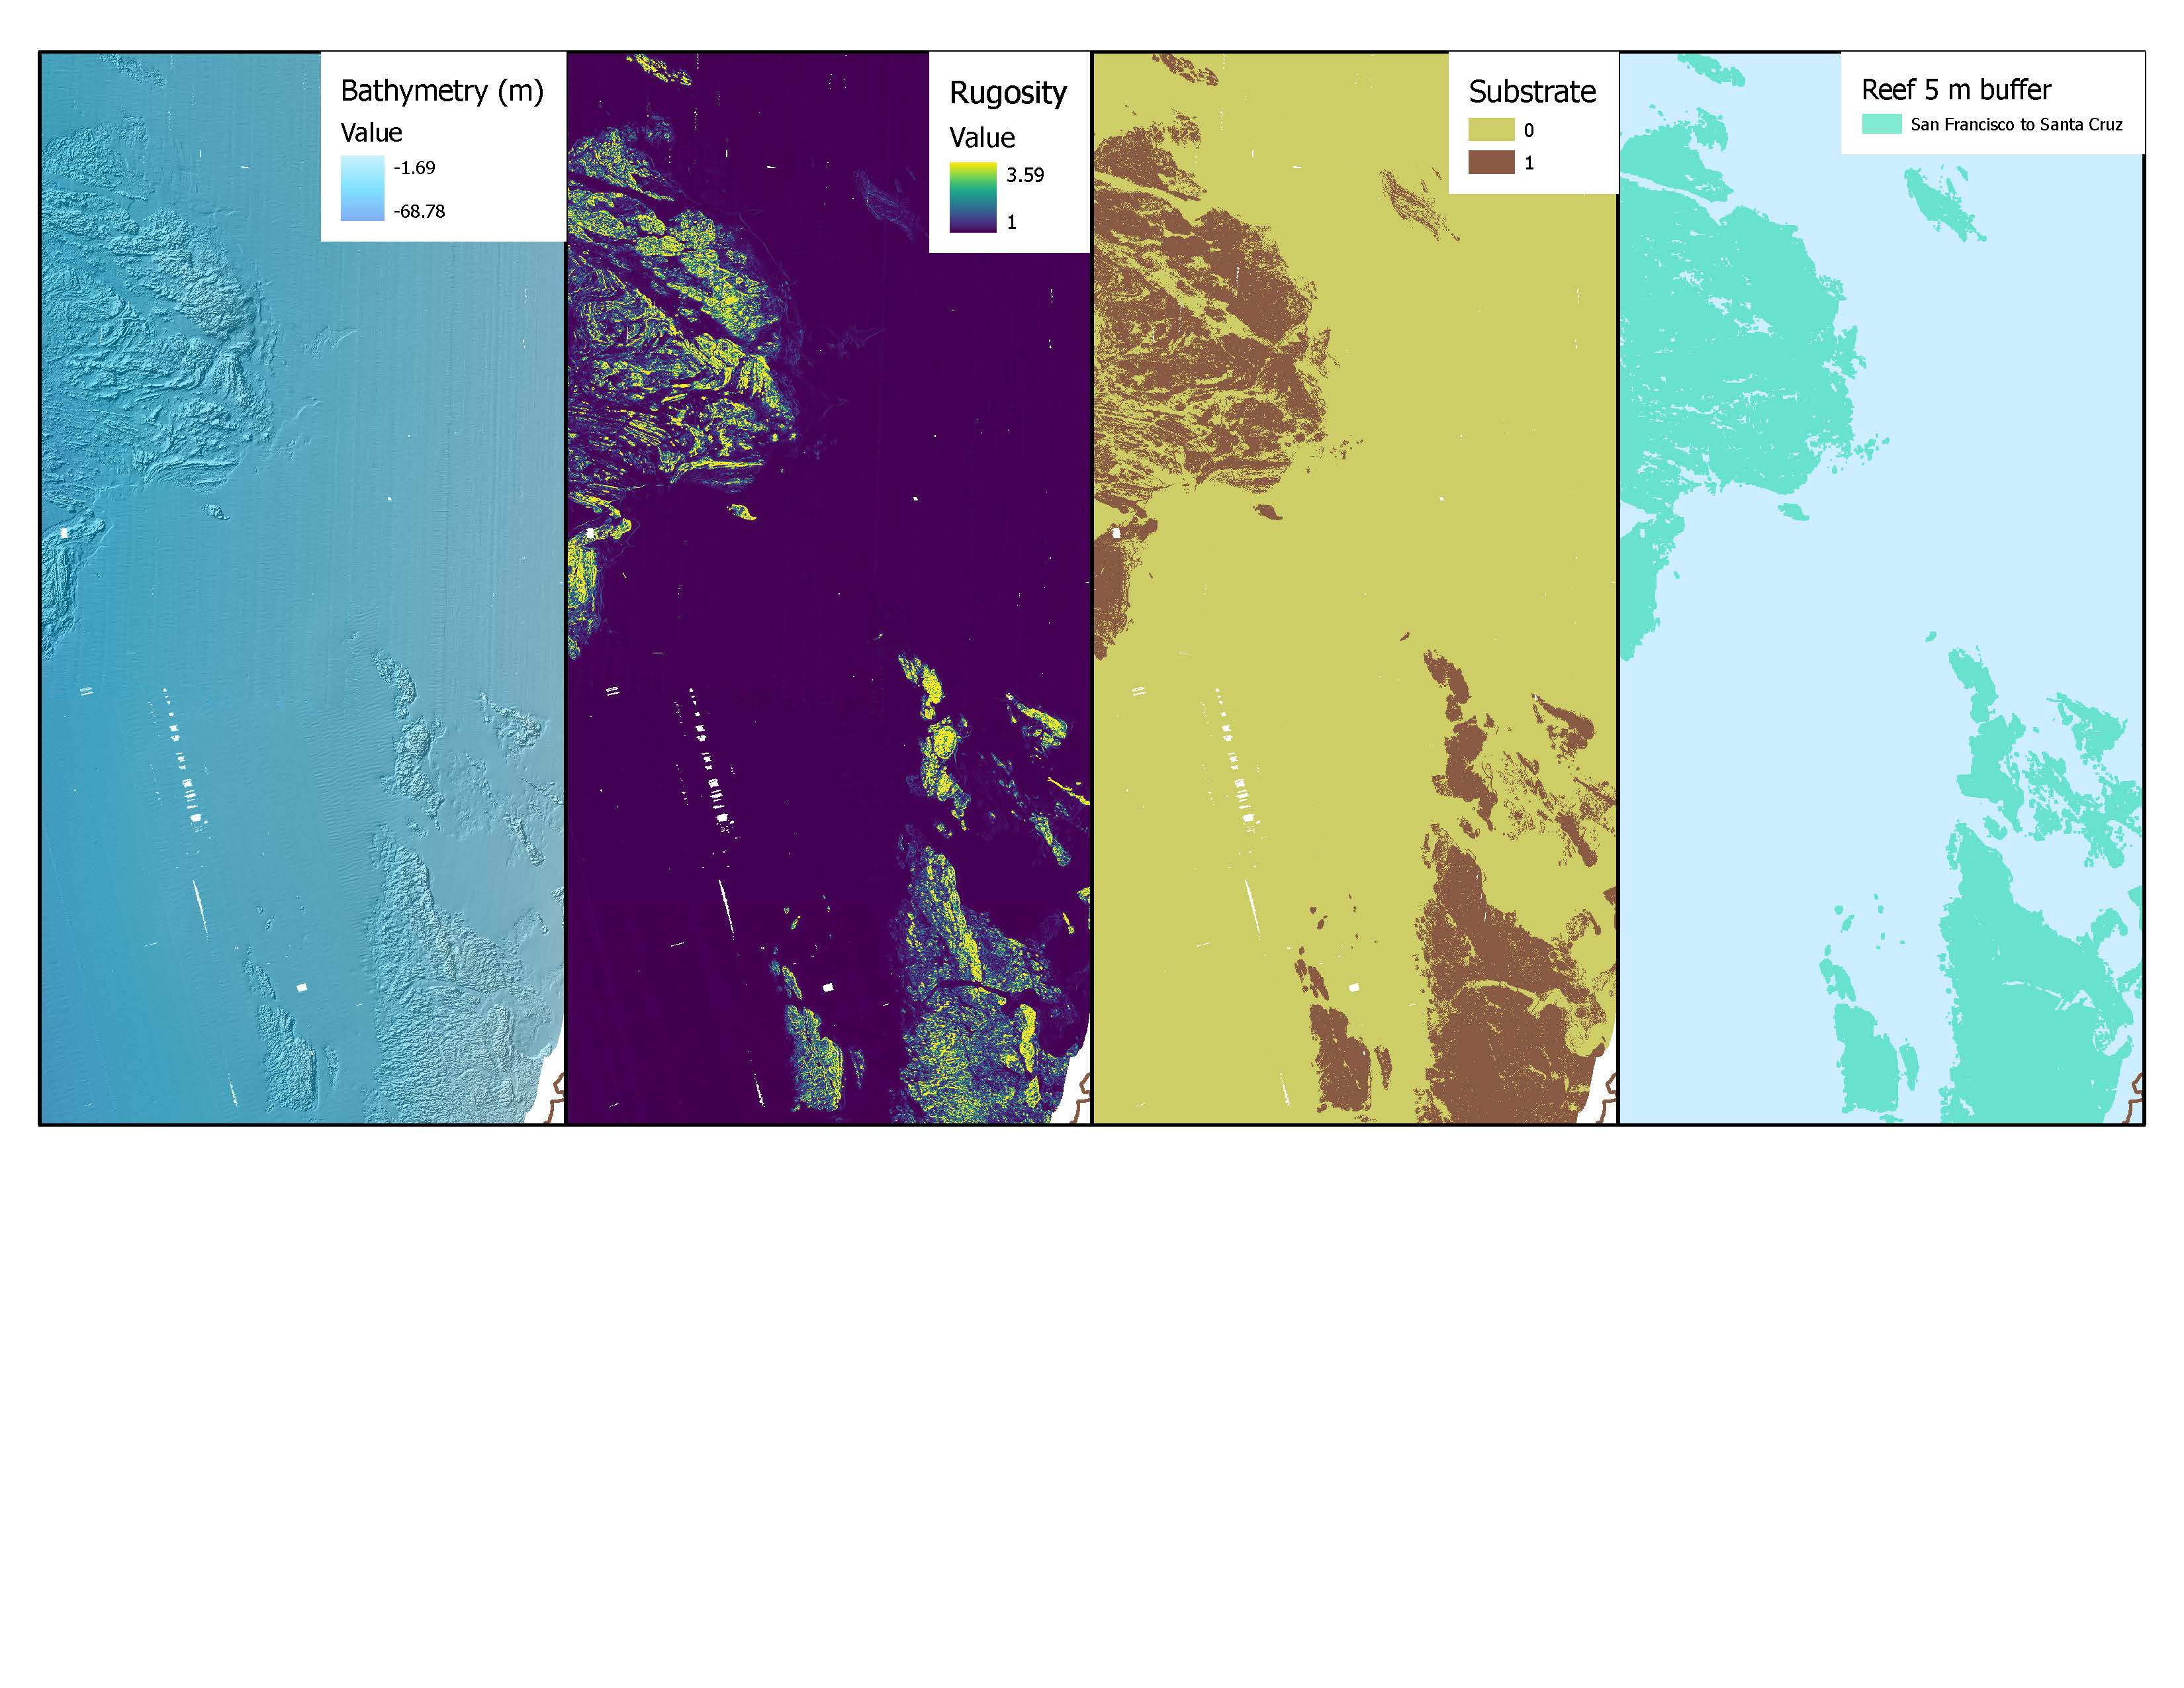
\includegraphics{figures/map_2.jpg}

}

\caption{\label{fig-map2}A example of the high resolution bathymetric
data and components of bathymetry and rugosity used to define rough
versus smooth substrate (where hard substrate is denoted by 1). The far
right panel displays the hard substrate with the added 5 m buffer to
represent the rocky reef habitat.}

\end{figure}

\begin{figure}

{\centering 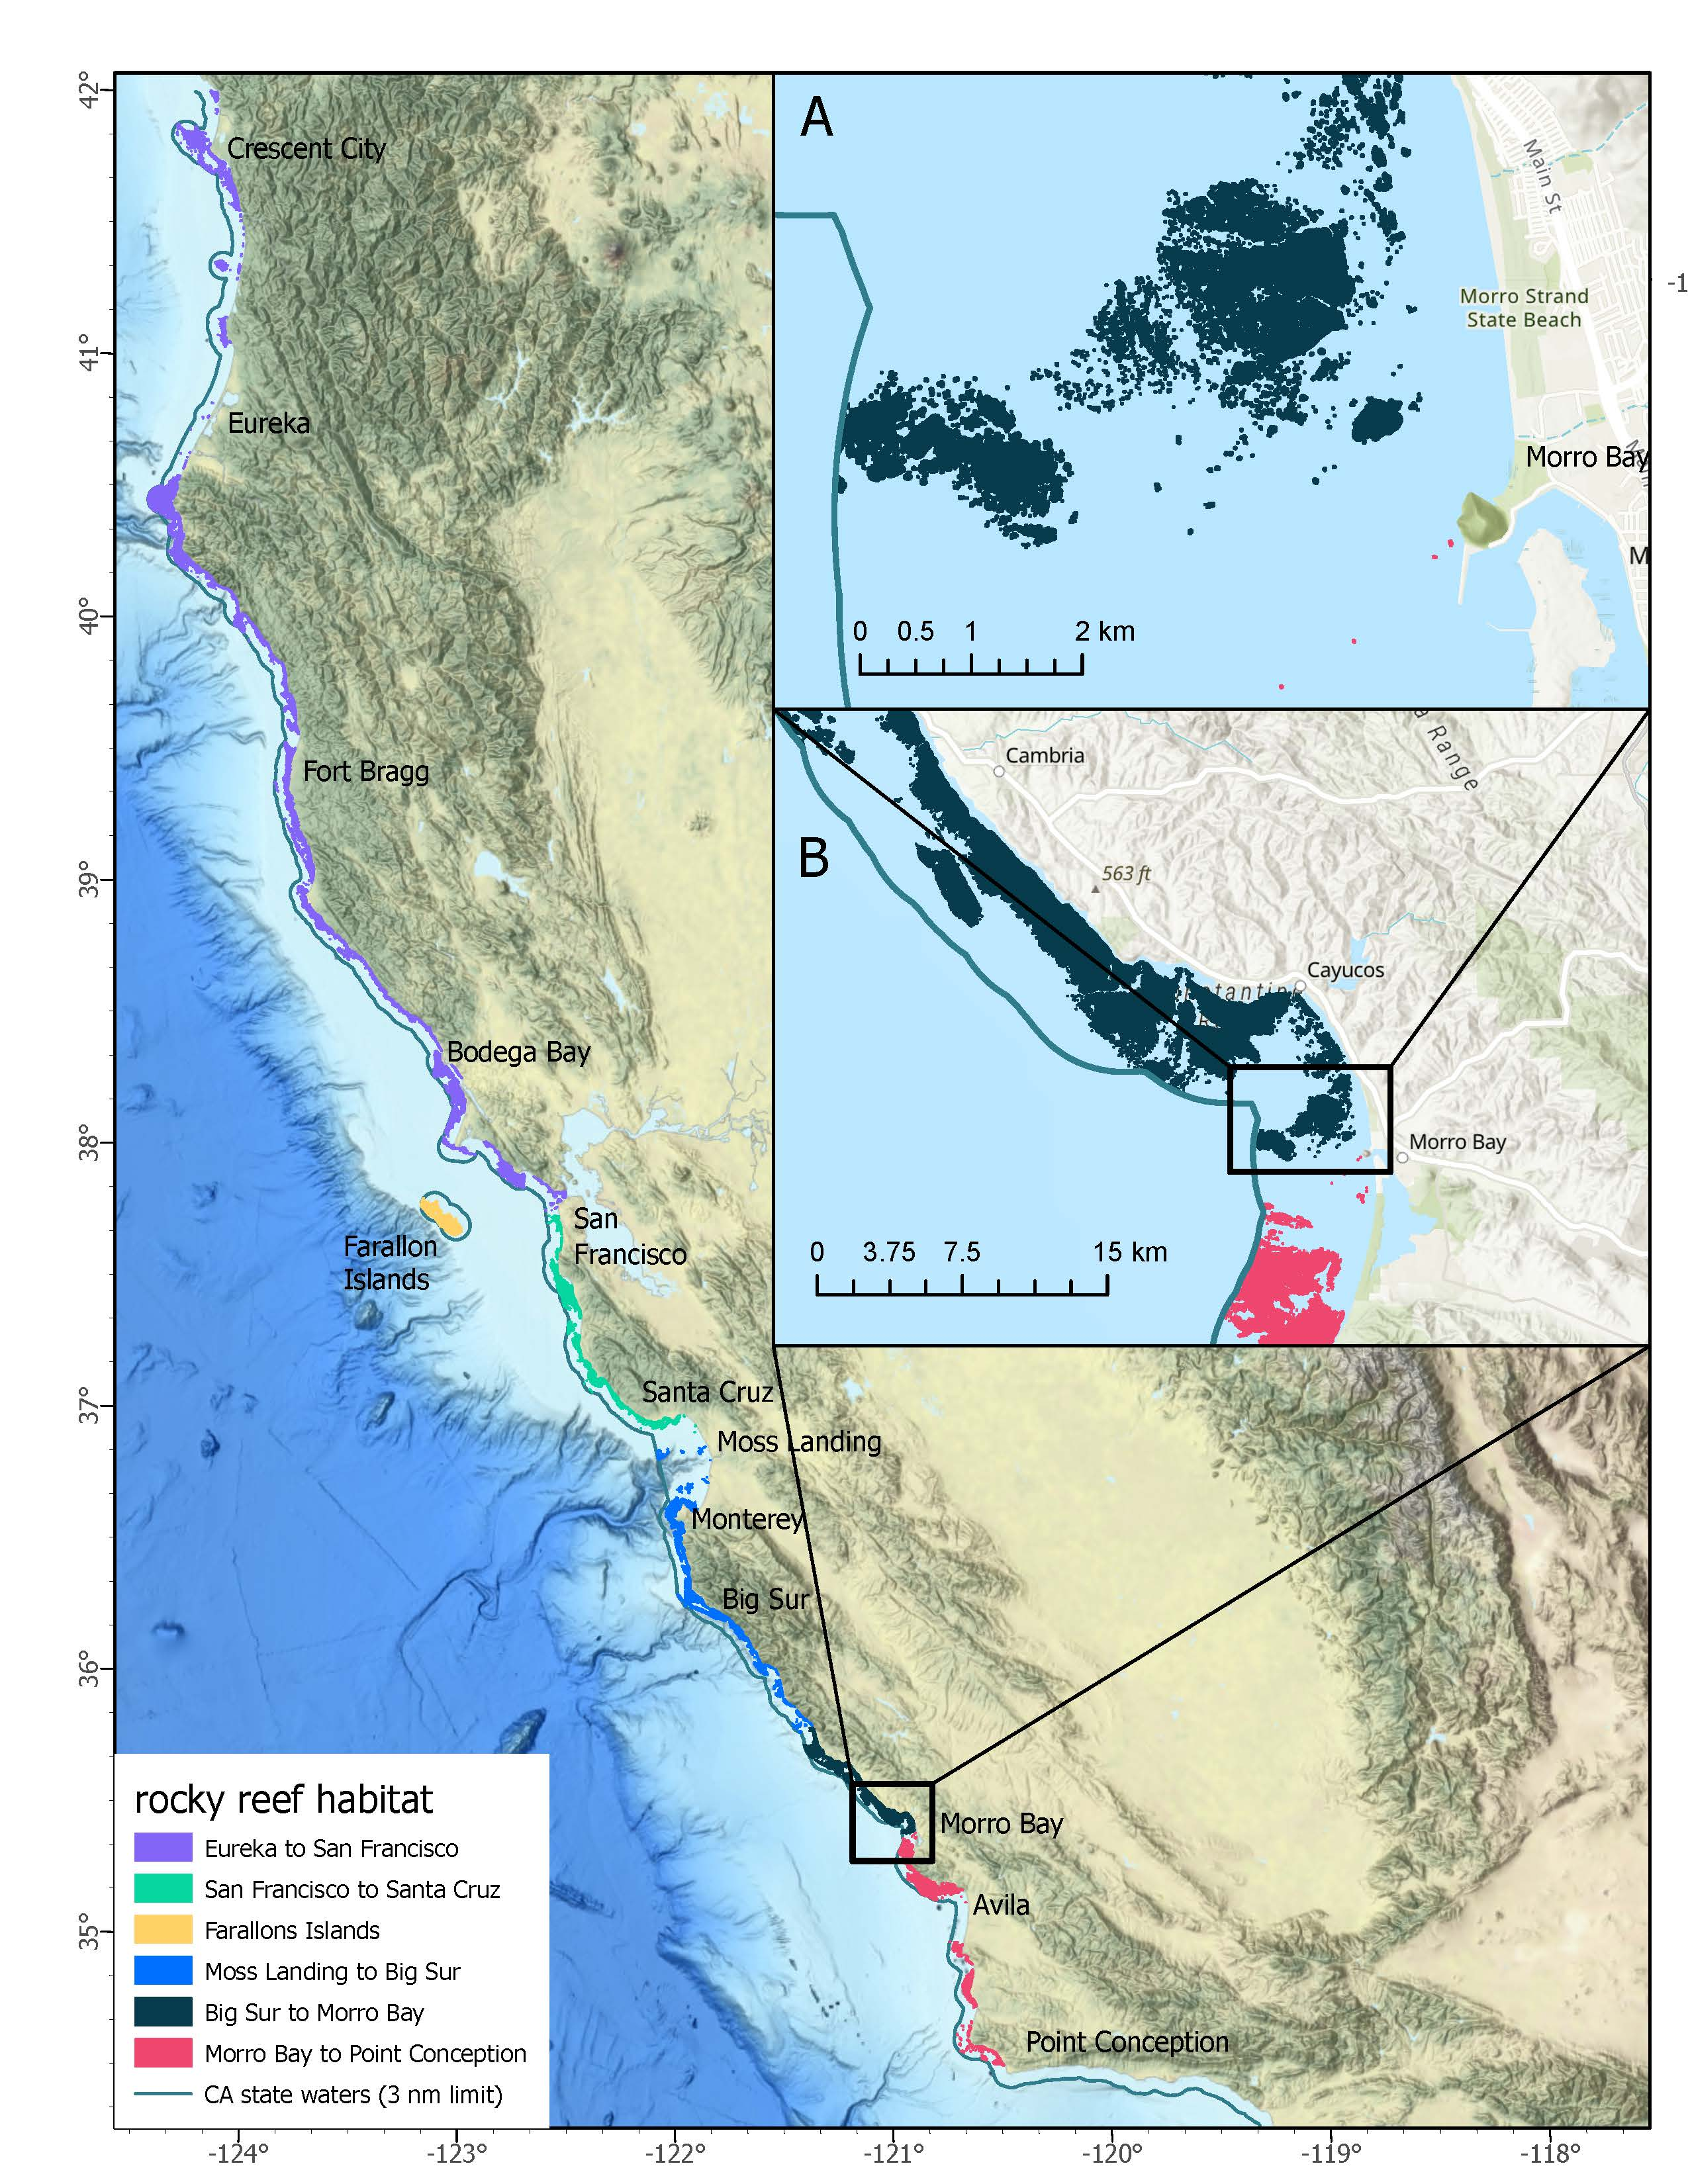
\includegraphics{figures/map.jpg}

}

\caption{\label{fig-map}A maps of California state waters north of Point
Conception colored by the aggregated areas of rocky reef habitat,
including inset A depicting the rocky reef habitat in relation to 3 nm
state water boundary state waters and inset B showing the high
resolution rocky habitat in the area.}

\end{figure}

\begin{figure}

{\centering \includegraphics{figures/percentpositives_map.jpg}

}

\caption{\label{fig-percentpos}The percent of drifts that retained the
target species, within grouped areas of rocky habitat over all years of
the time series. The grey dashed lines represent the aggregated rocky
habitat used to develop an index of abundance.}

\end{figure}

\begin{figure}

{\centering 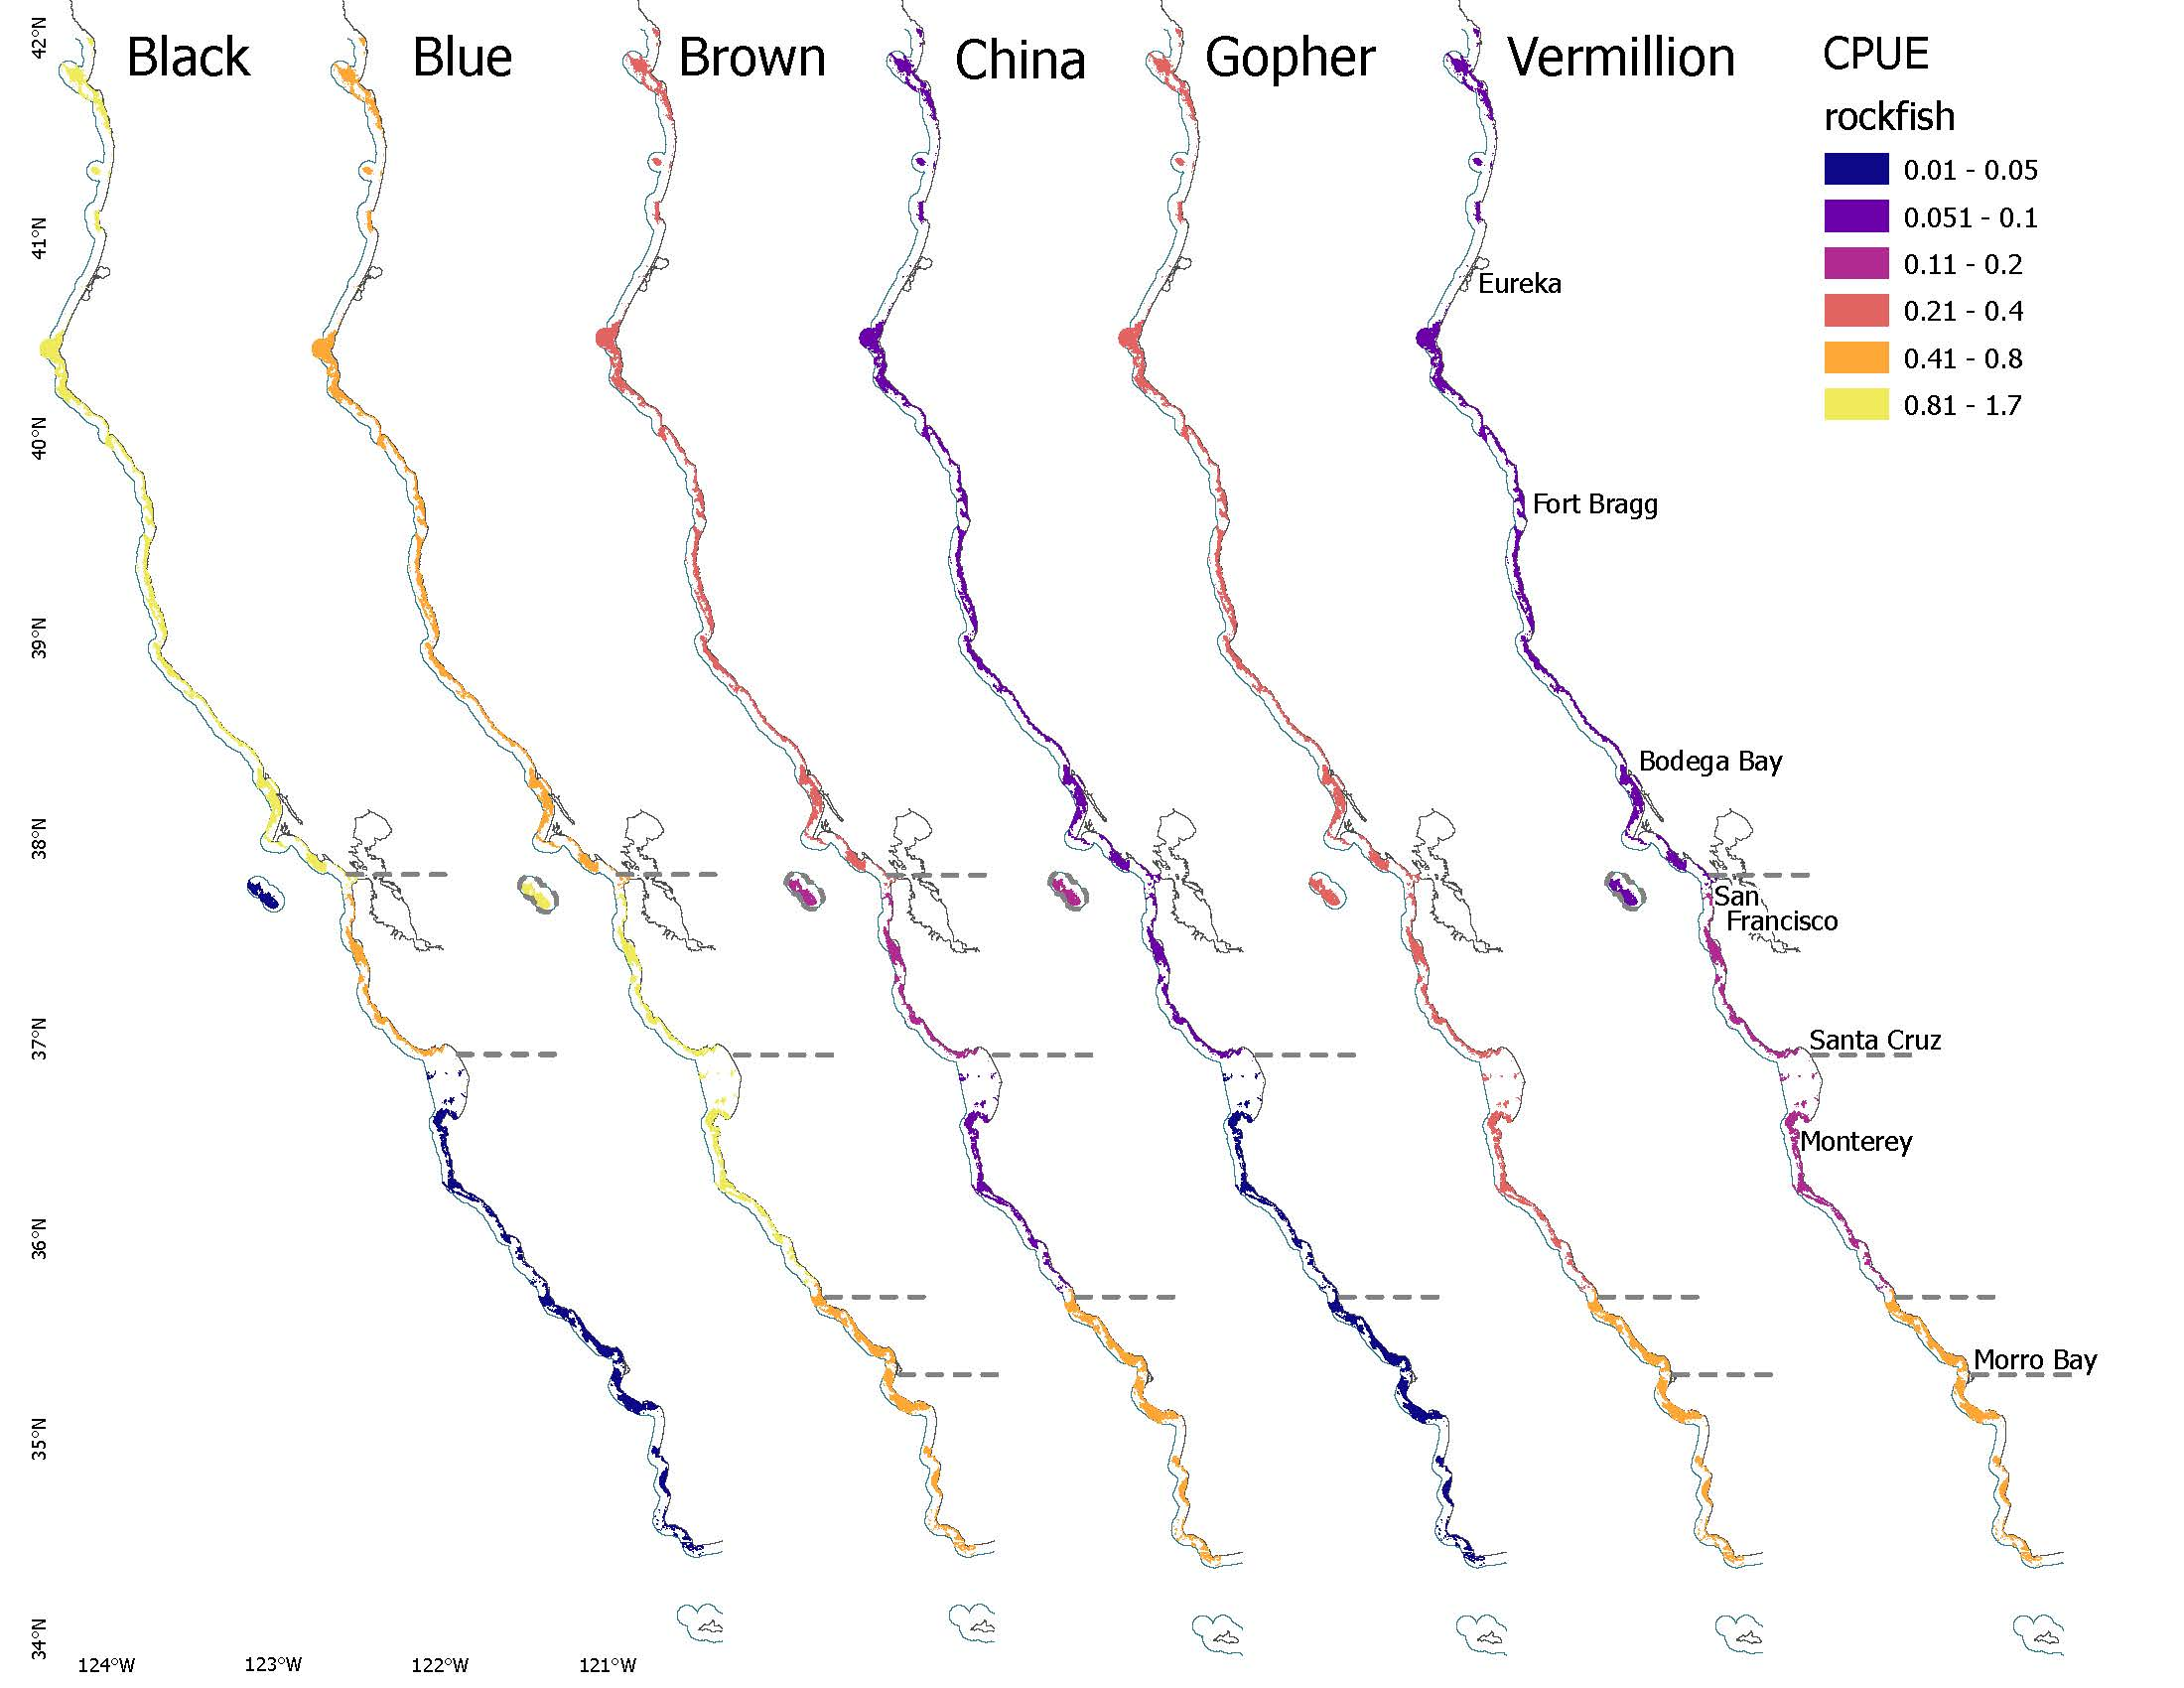
\includegraphics{figures/CPUE_map.jpg}

}

\caption{\label{fig-cpue}The average CPUE across all years of the time
series for each of the six species. The grey dashed lines represent the
aggregated rocky habitat used to develop an index of abundance.}

\end{figure}

\begin{figure}

\begin{minipage}[t]{0.50\linewidth}

{\centering 

\raisebox{-\height}{

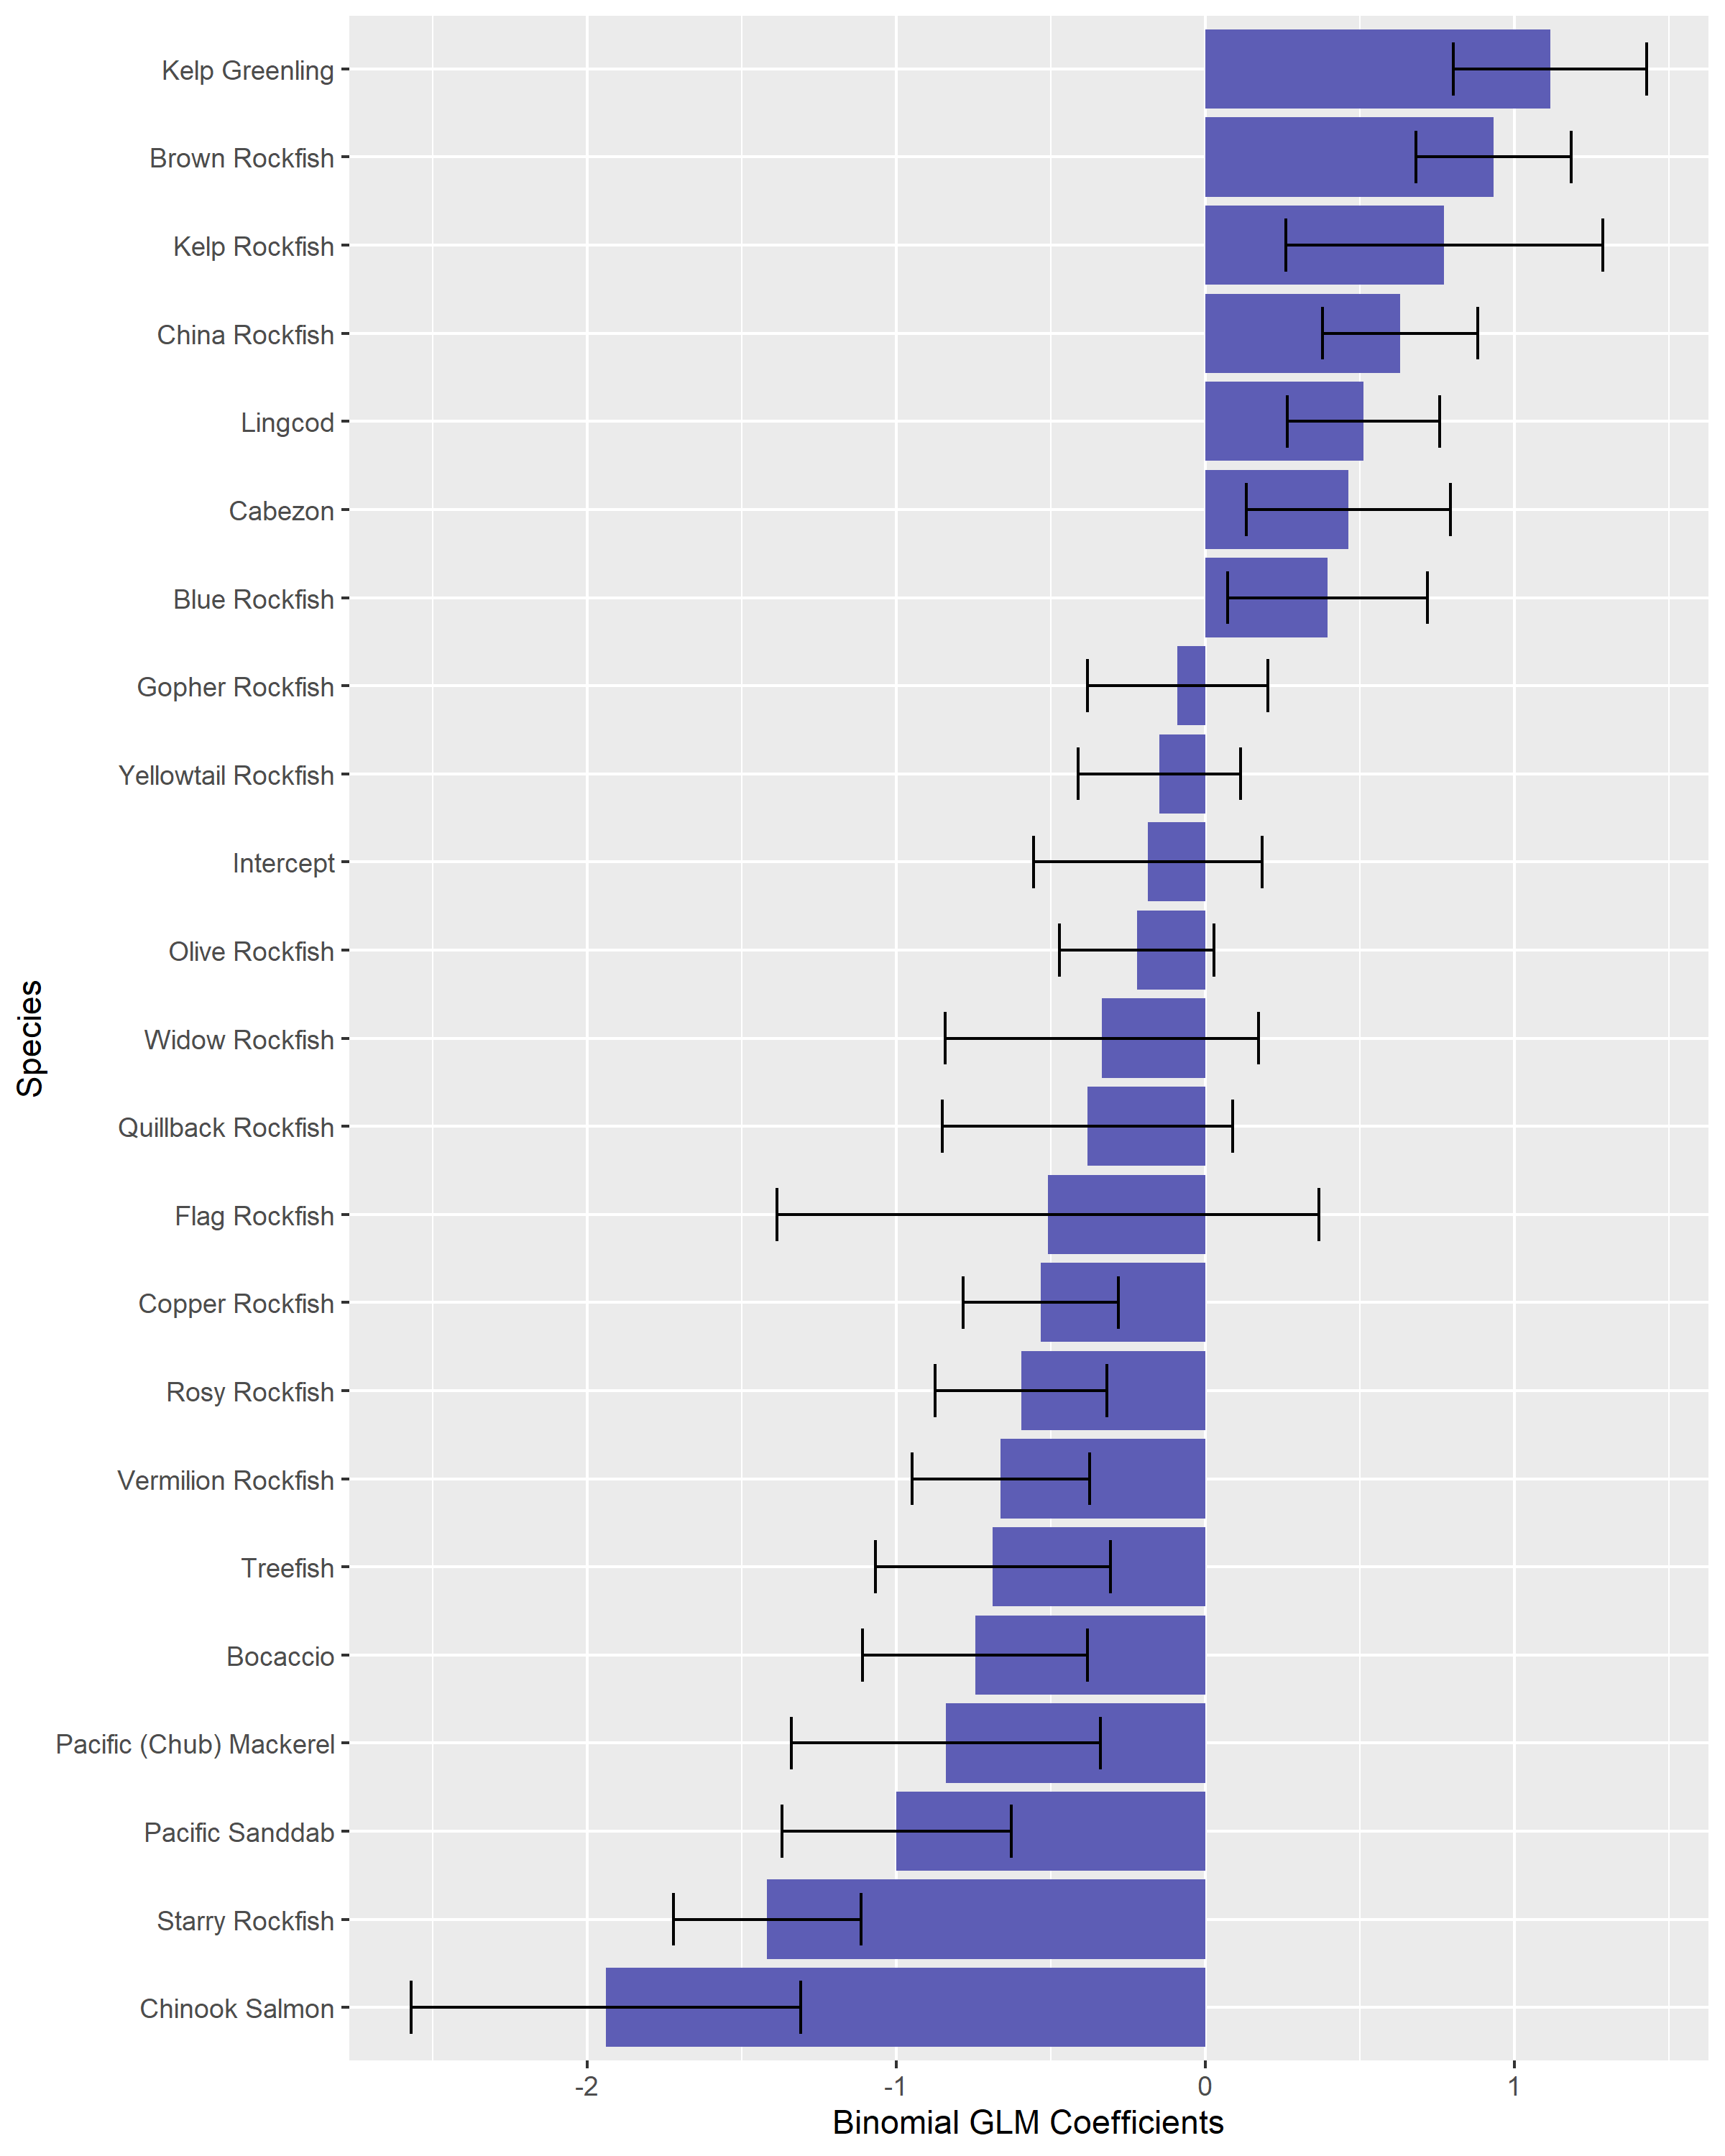
\includegraphics[width=2.7in,height=\textheight]{figures/black_trip_sm.png}

}

}

\subcaption{\label{fig-black-tripsm}Black rockfish trip-level}
\end{minipage}%
%
\begin{minipage}[t]{0.50\linewidth}

{\centering 

\raisebox{-\height}{

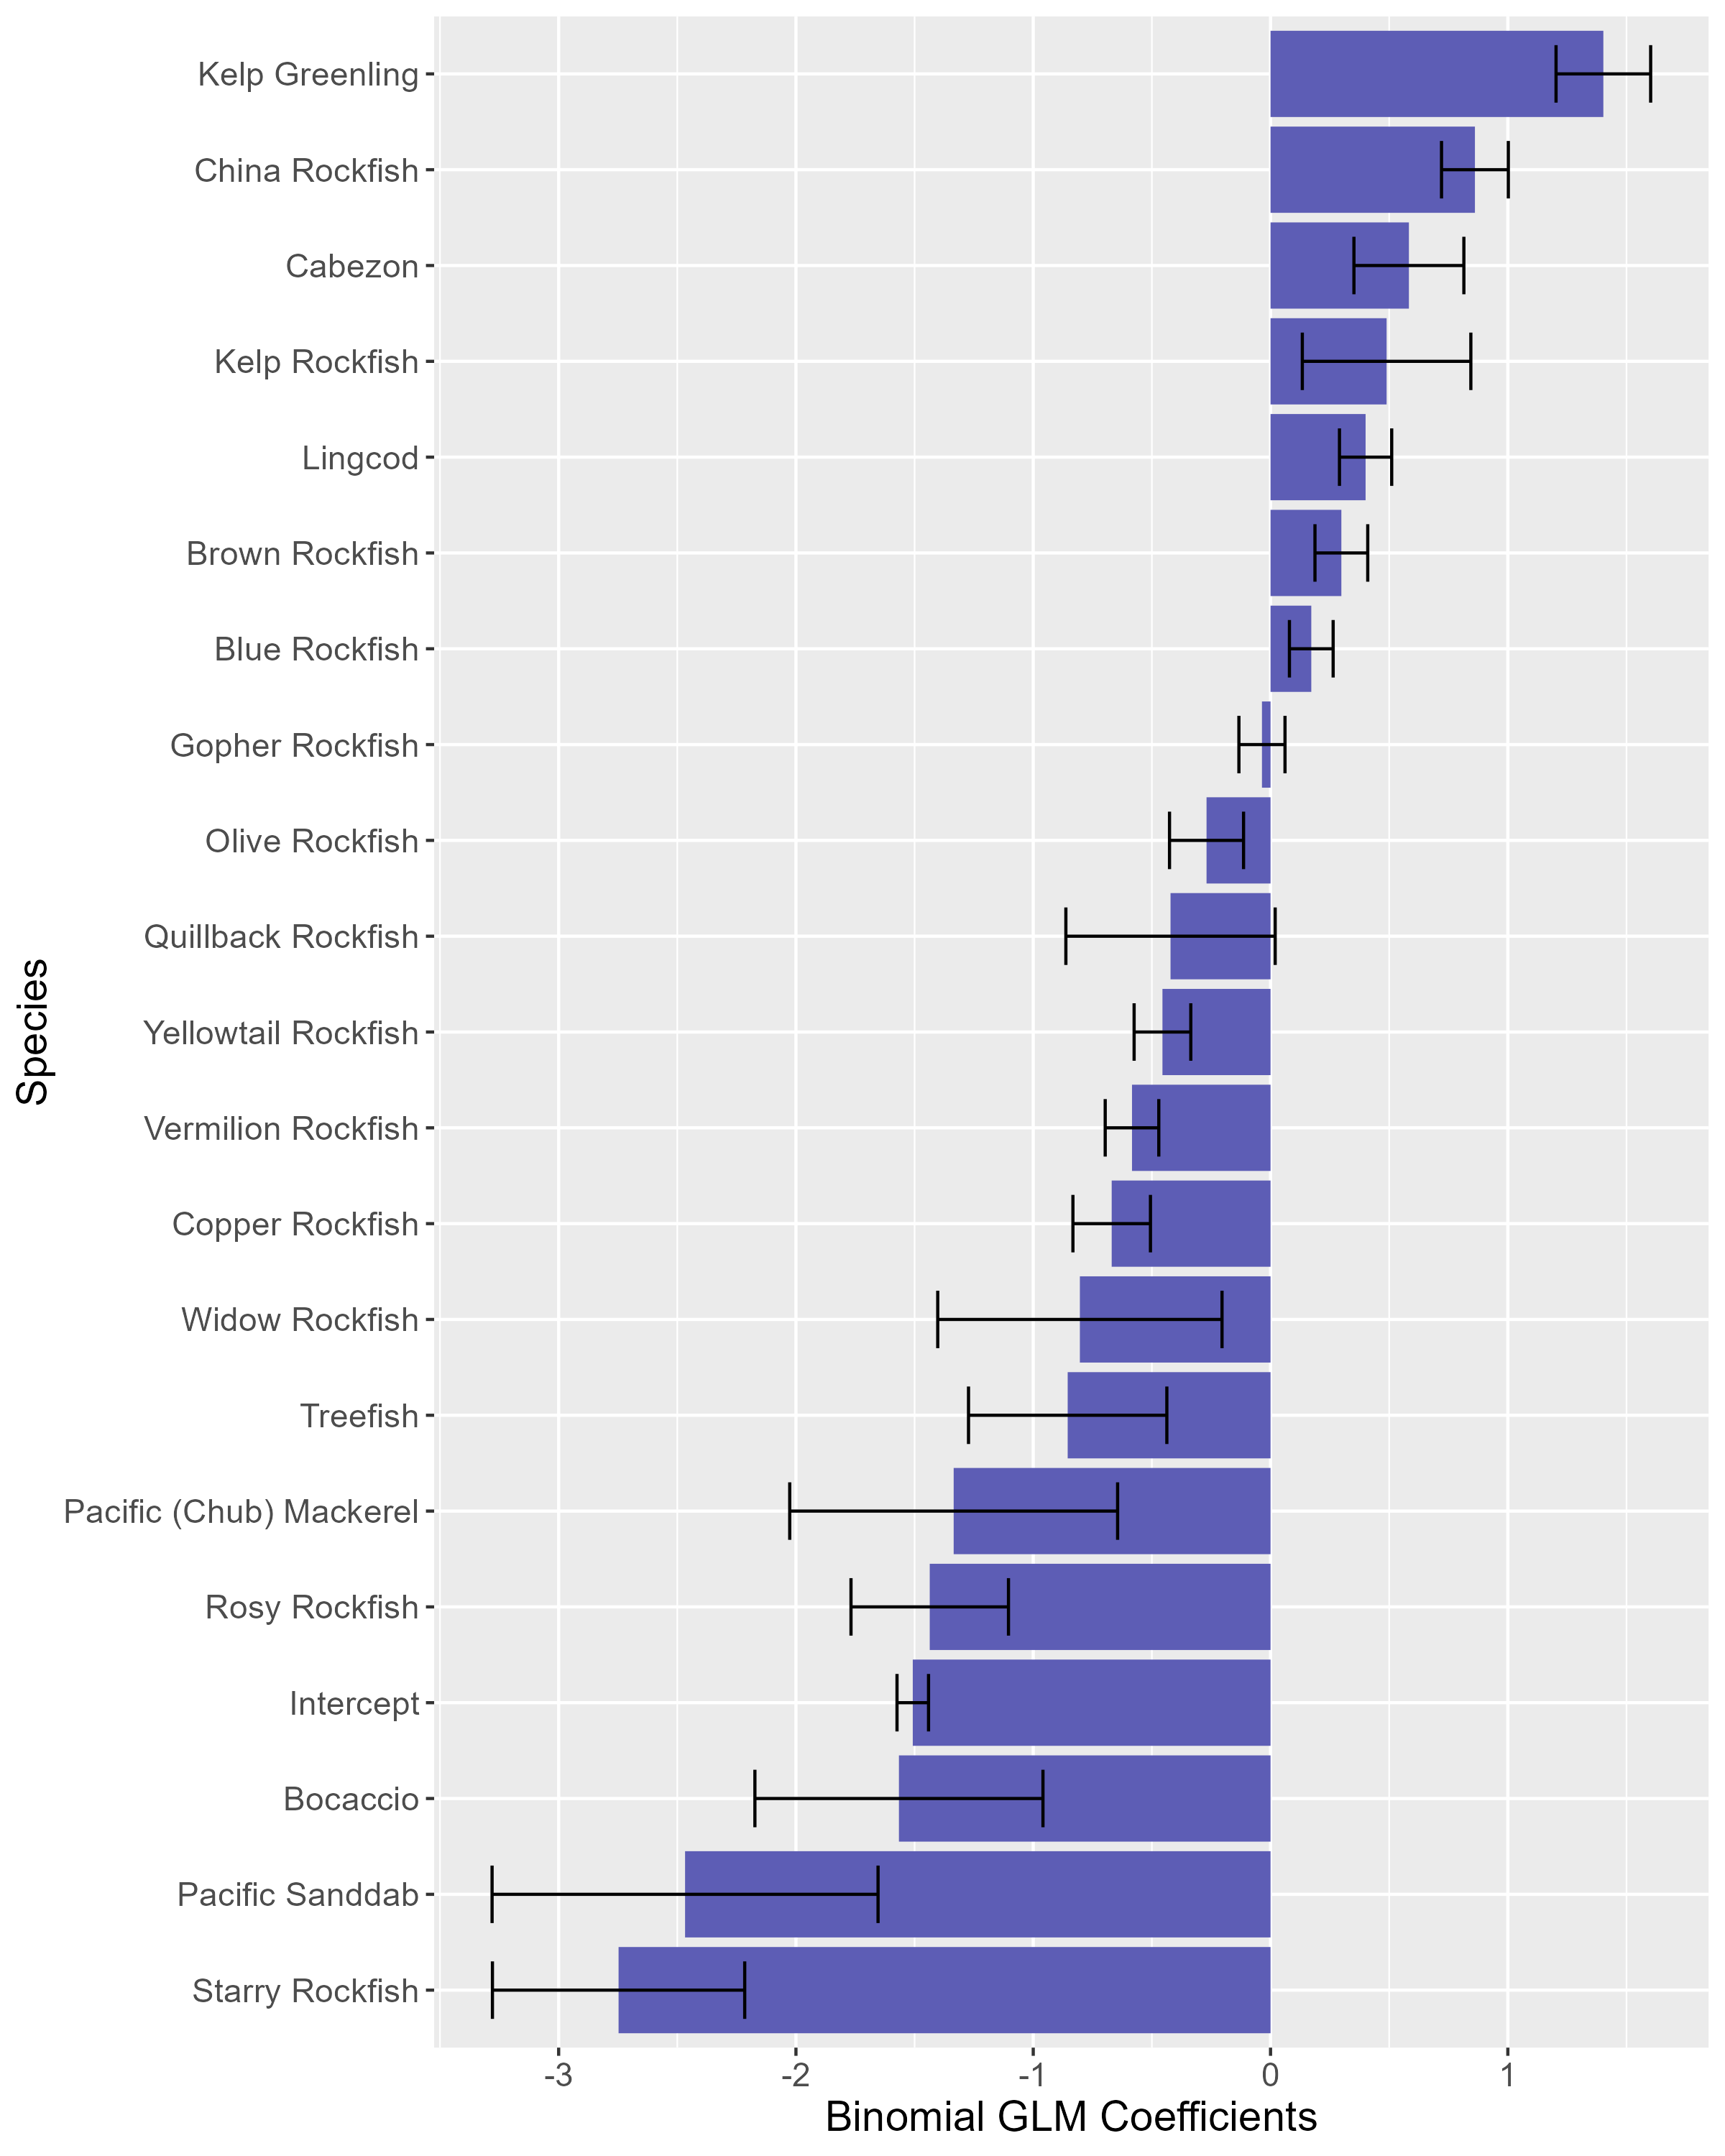
\includegraphics[width=2.7in,height=\textheight]{figures/black_drift_sm.png}

}

}

\subcaption{\label{fig-black-driftsm}Black rockfish drift-level}
\end{minipage}%
\newline
\begin{minipage}[t]{0.50\linewidth}

{\centering 

\raisebox{-\height}{

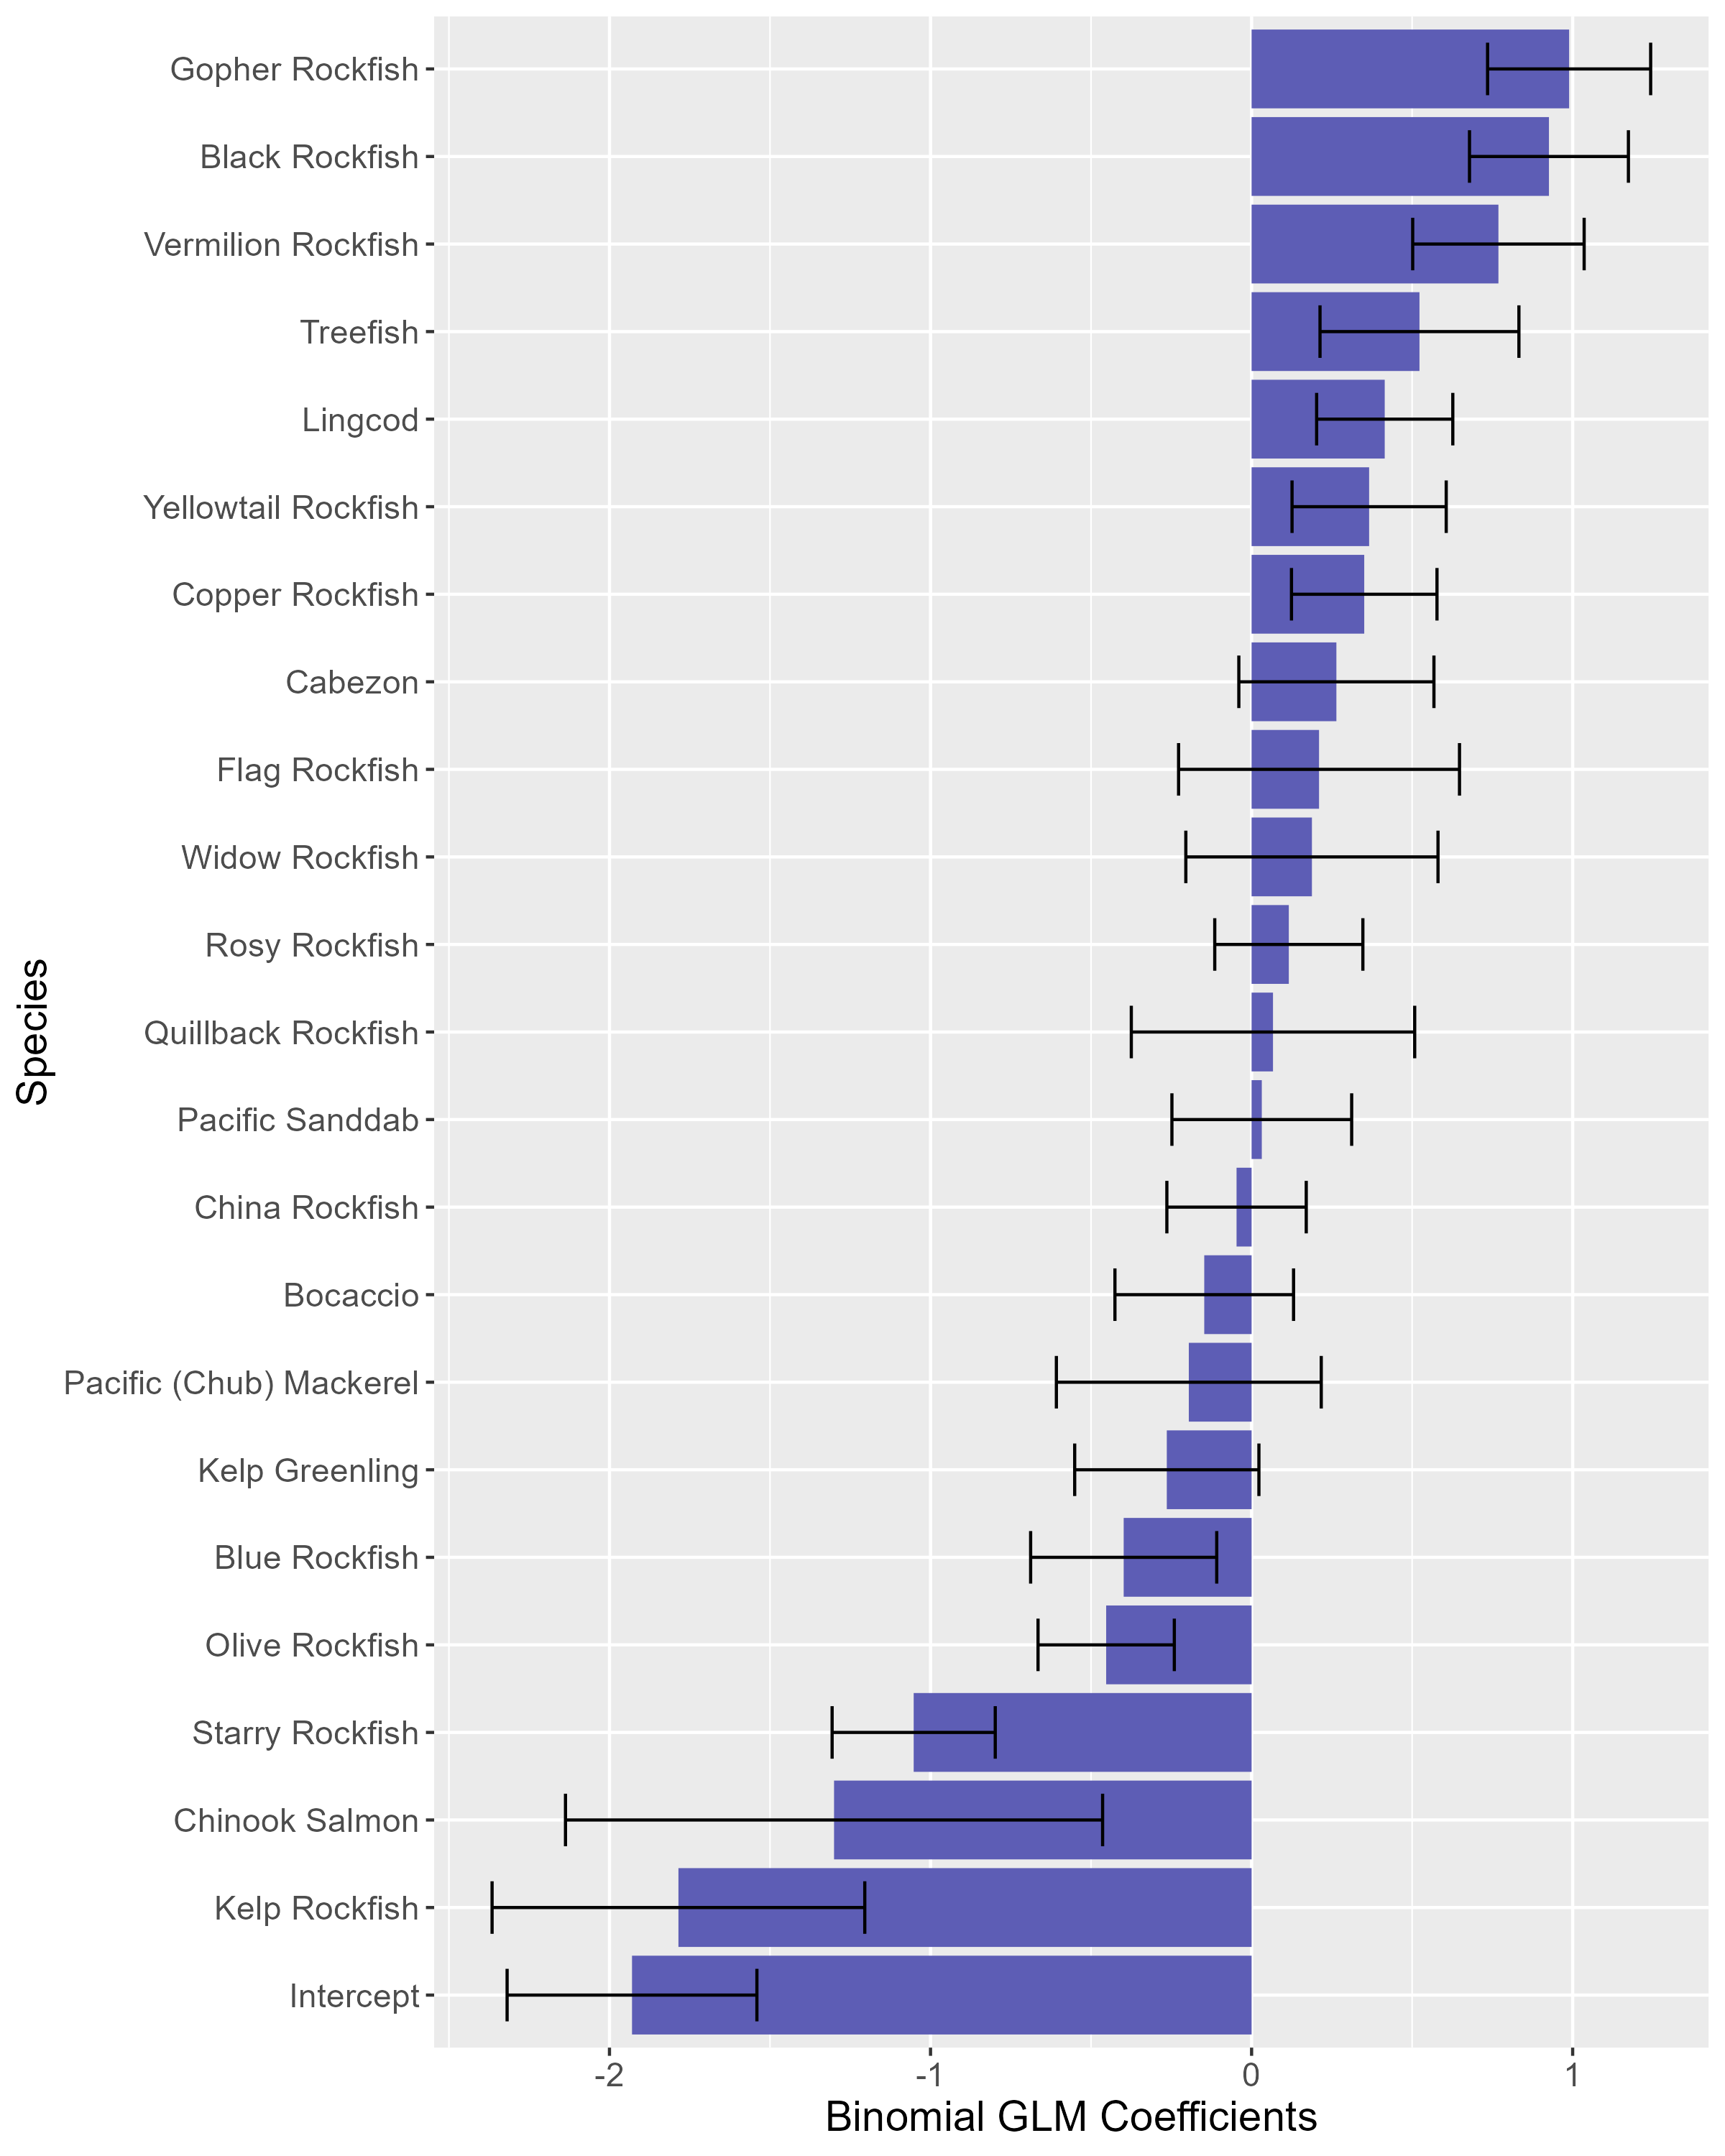
\includegraphics[width=2.7in,height=\textheight]{figures/brown_trip_sm.png}

}

}

\subcaption{\label{fig-brown-tripsm}Brown rockfish trip-level}
\end{minipage}%
%
\begin{minipage}[t]{0.50\linewidth}

{\centering 

\raisebox{-\height}{

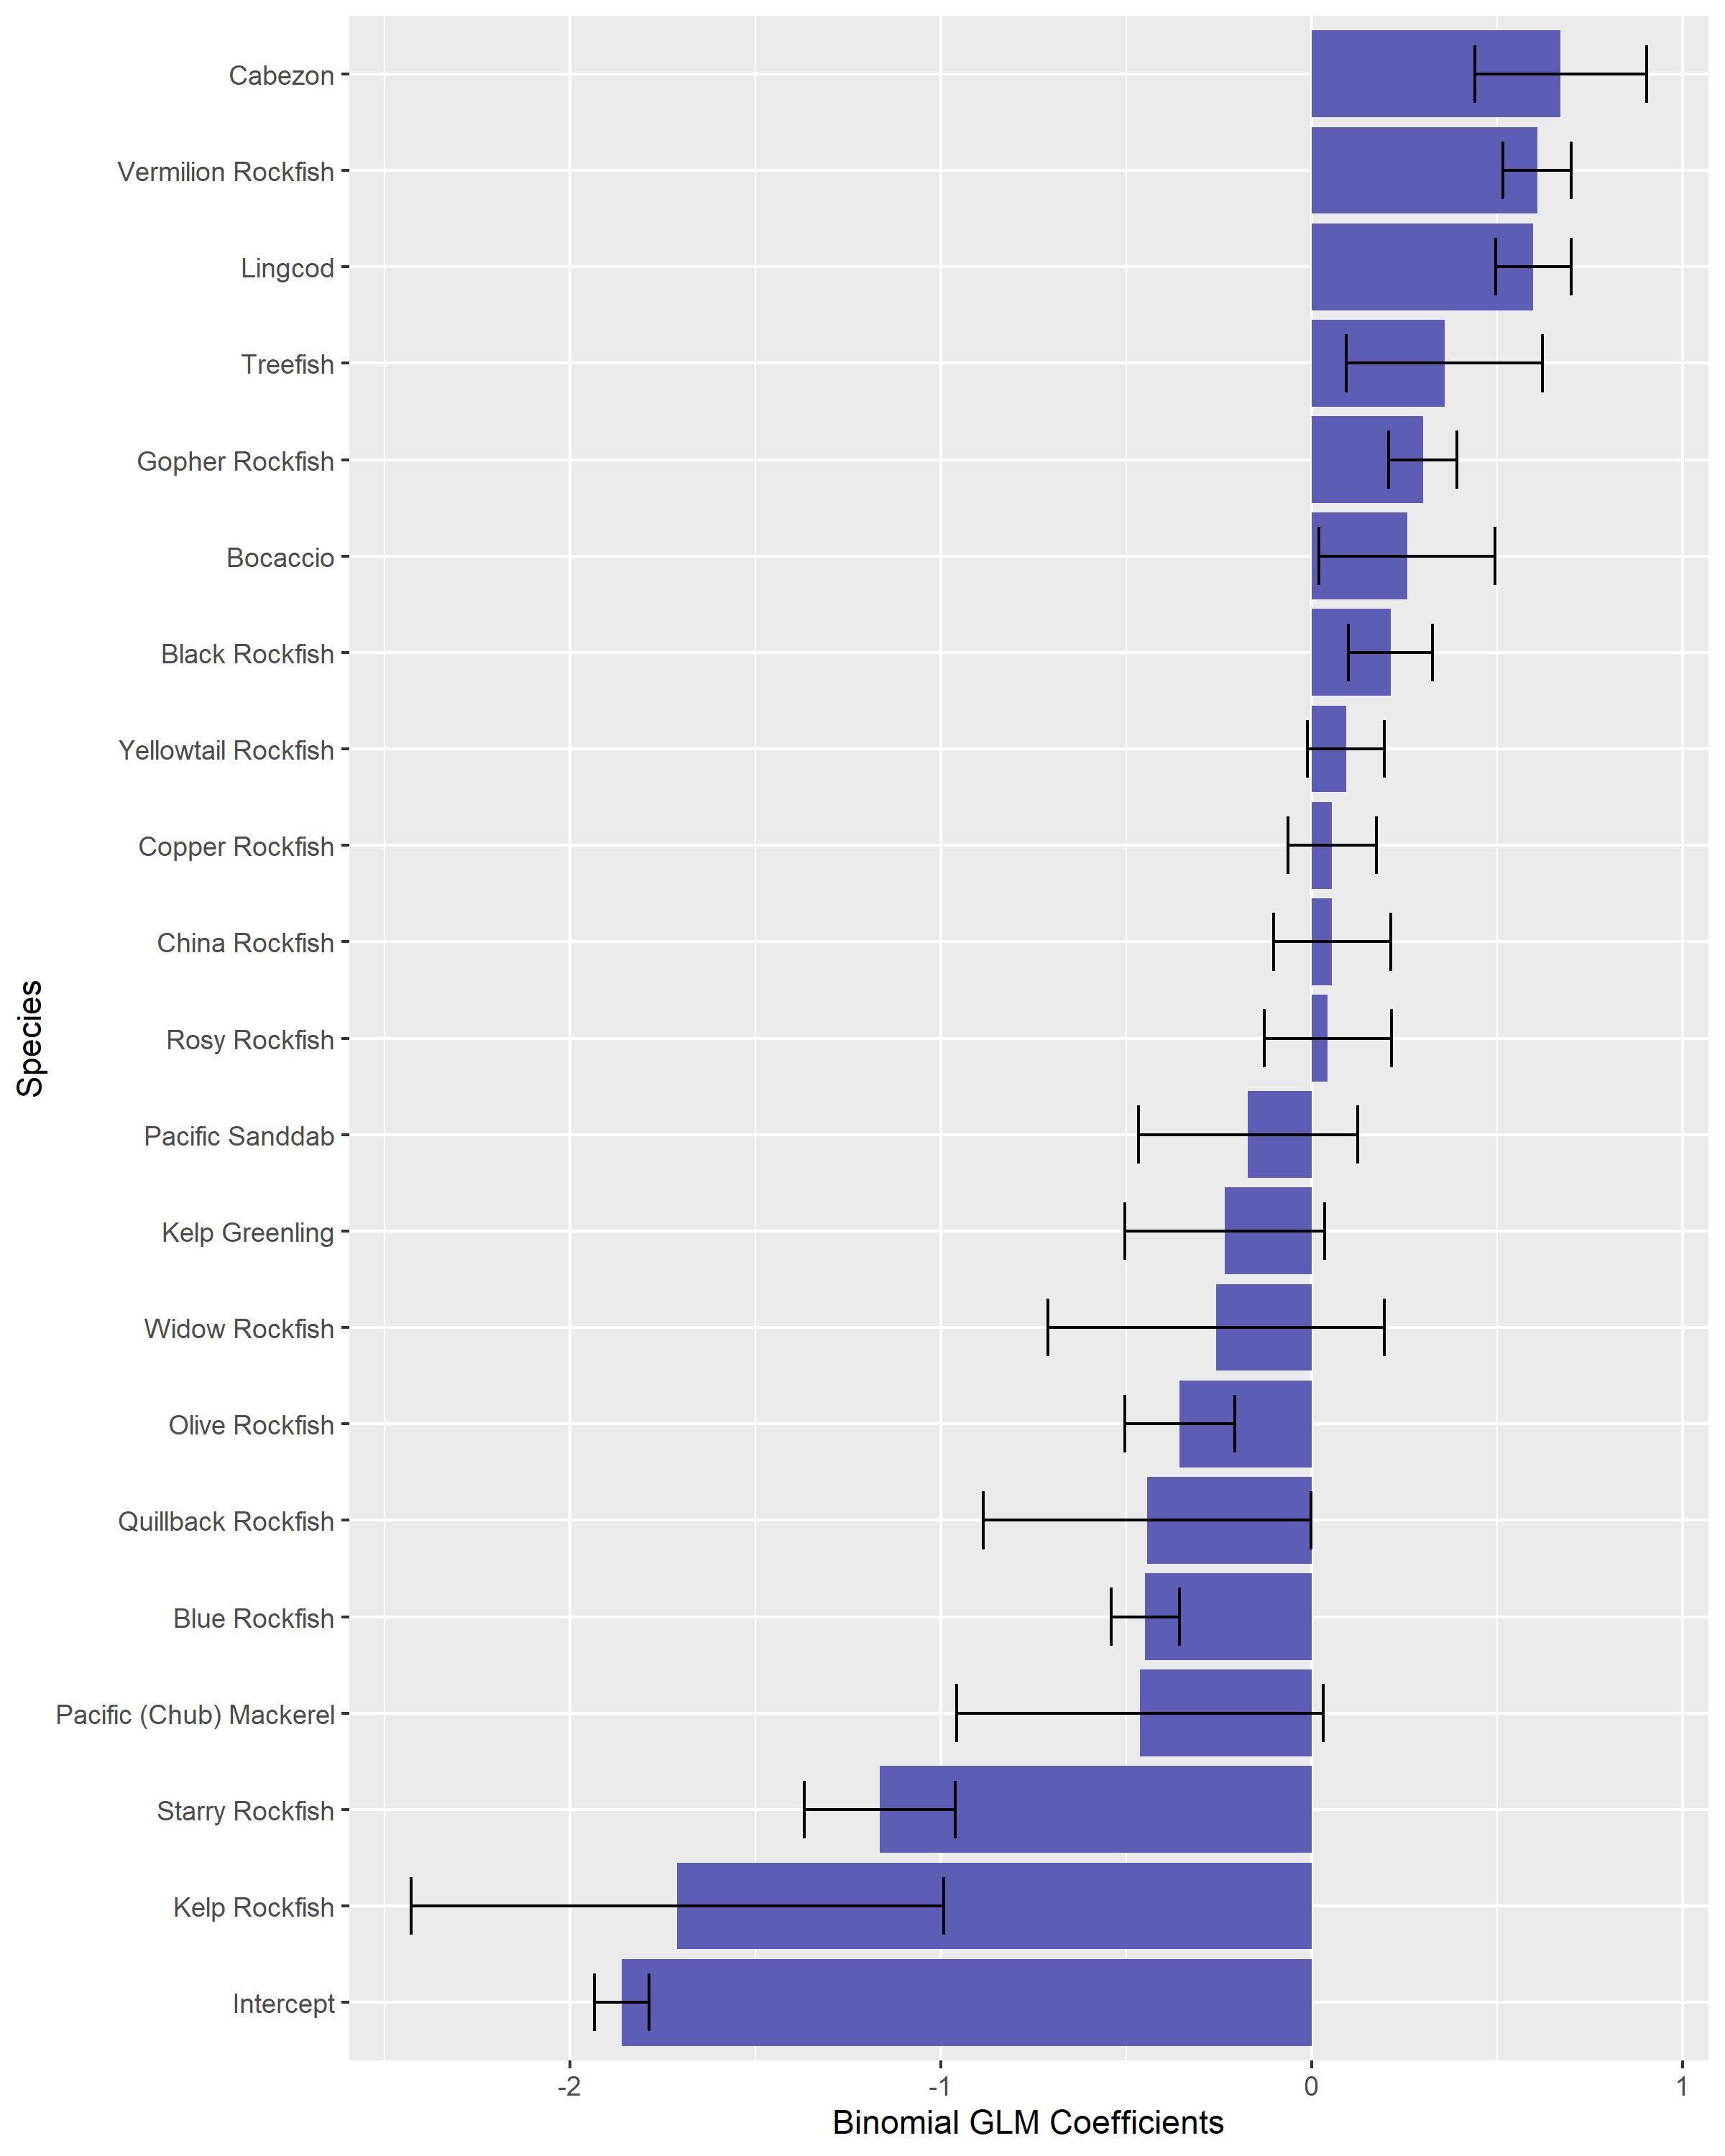
\includegraphics[width=2.7in,height=\textheight]{figures/brown_drift_sm.png}

}

}

\subcaption{\label{fig-brown-driftsm}Brown rockfish drift-level}
\end{minipage}%

\caption{\label{fig-sm}Examples of the species coefficients and 95\%
confidence intervals for the Stephens-MacCall filtering for black
rockfish and brown rockfish for the trip-level and drift-level data.}

\end{figure}

\begin{figure}

\begin{minipage}[t]{0.50\linewidth}

{\centering 

\raisebox{-\height}{

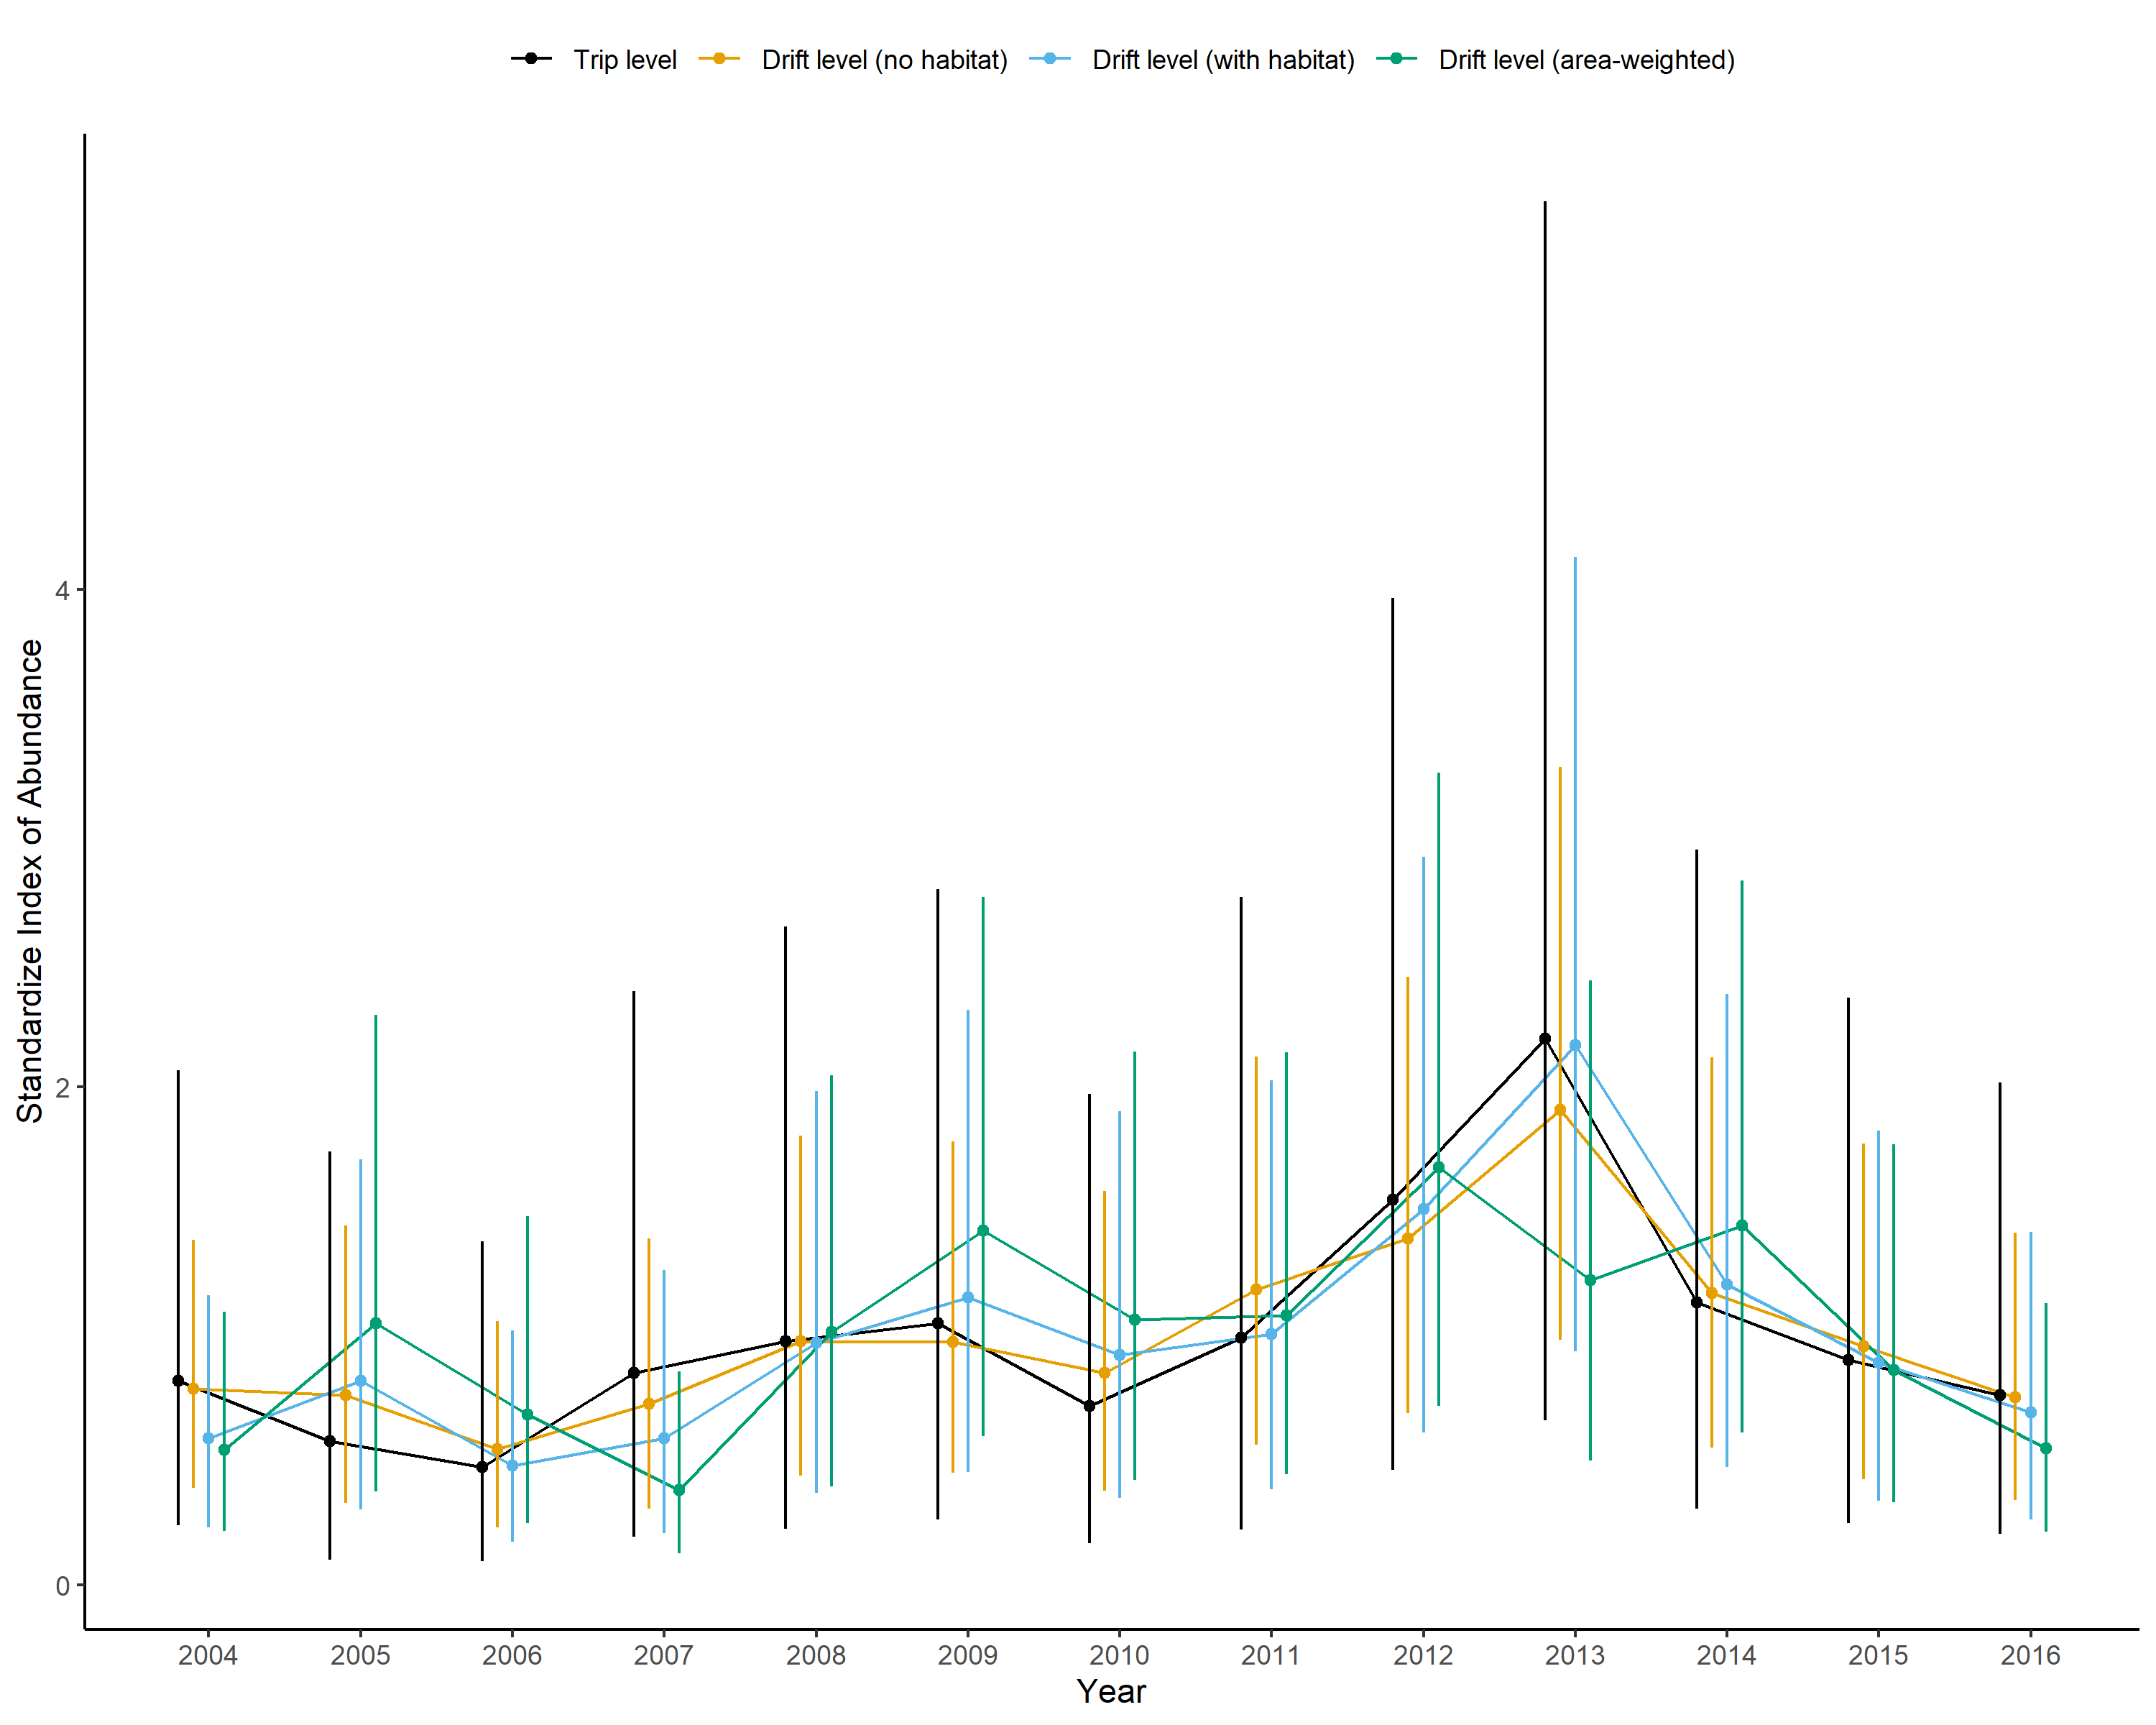
\includegraphics[width=3in,height=\textheight]{figures/black_indices.png}

}

}

\subcaption{\label{fig-black-indices}Black rockfish}
\end{minipage}%
%
\begin{minipage}[t]{0.50\linewidth}

{\centering 

\raisebox{-\height}{

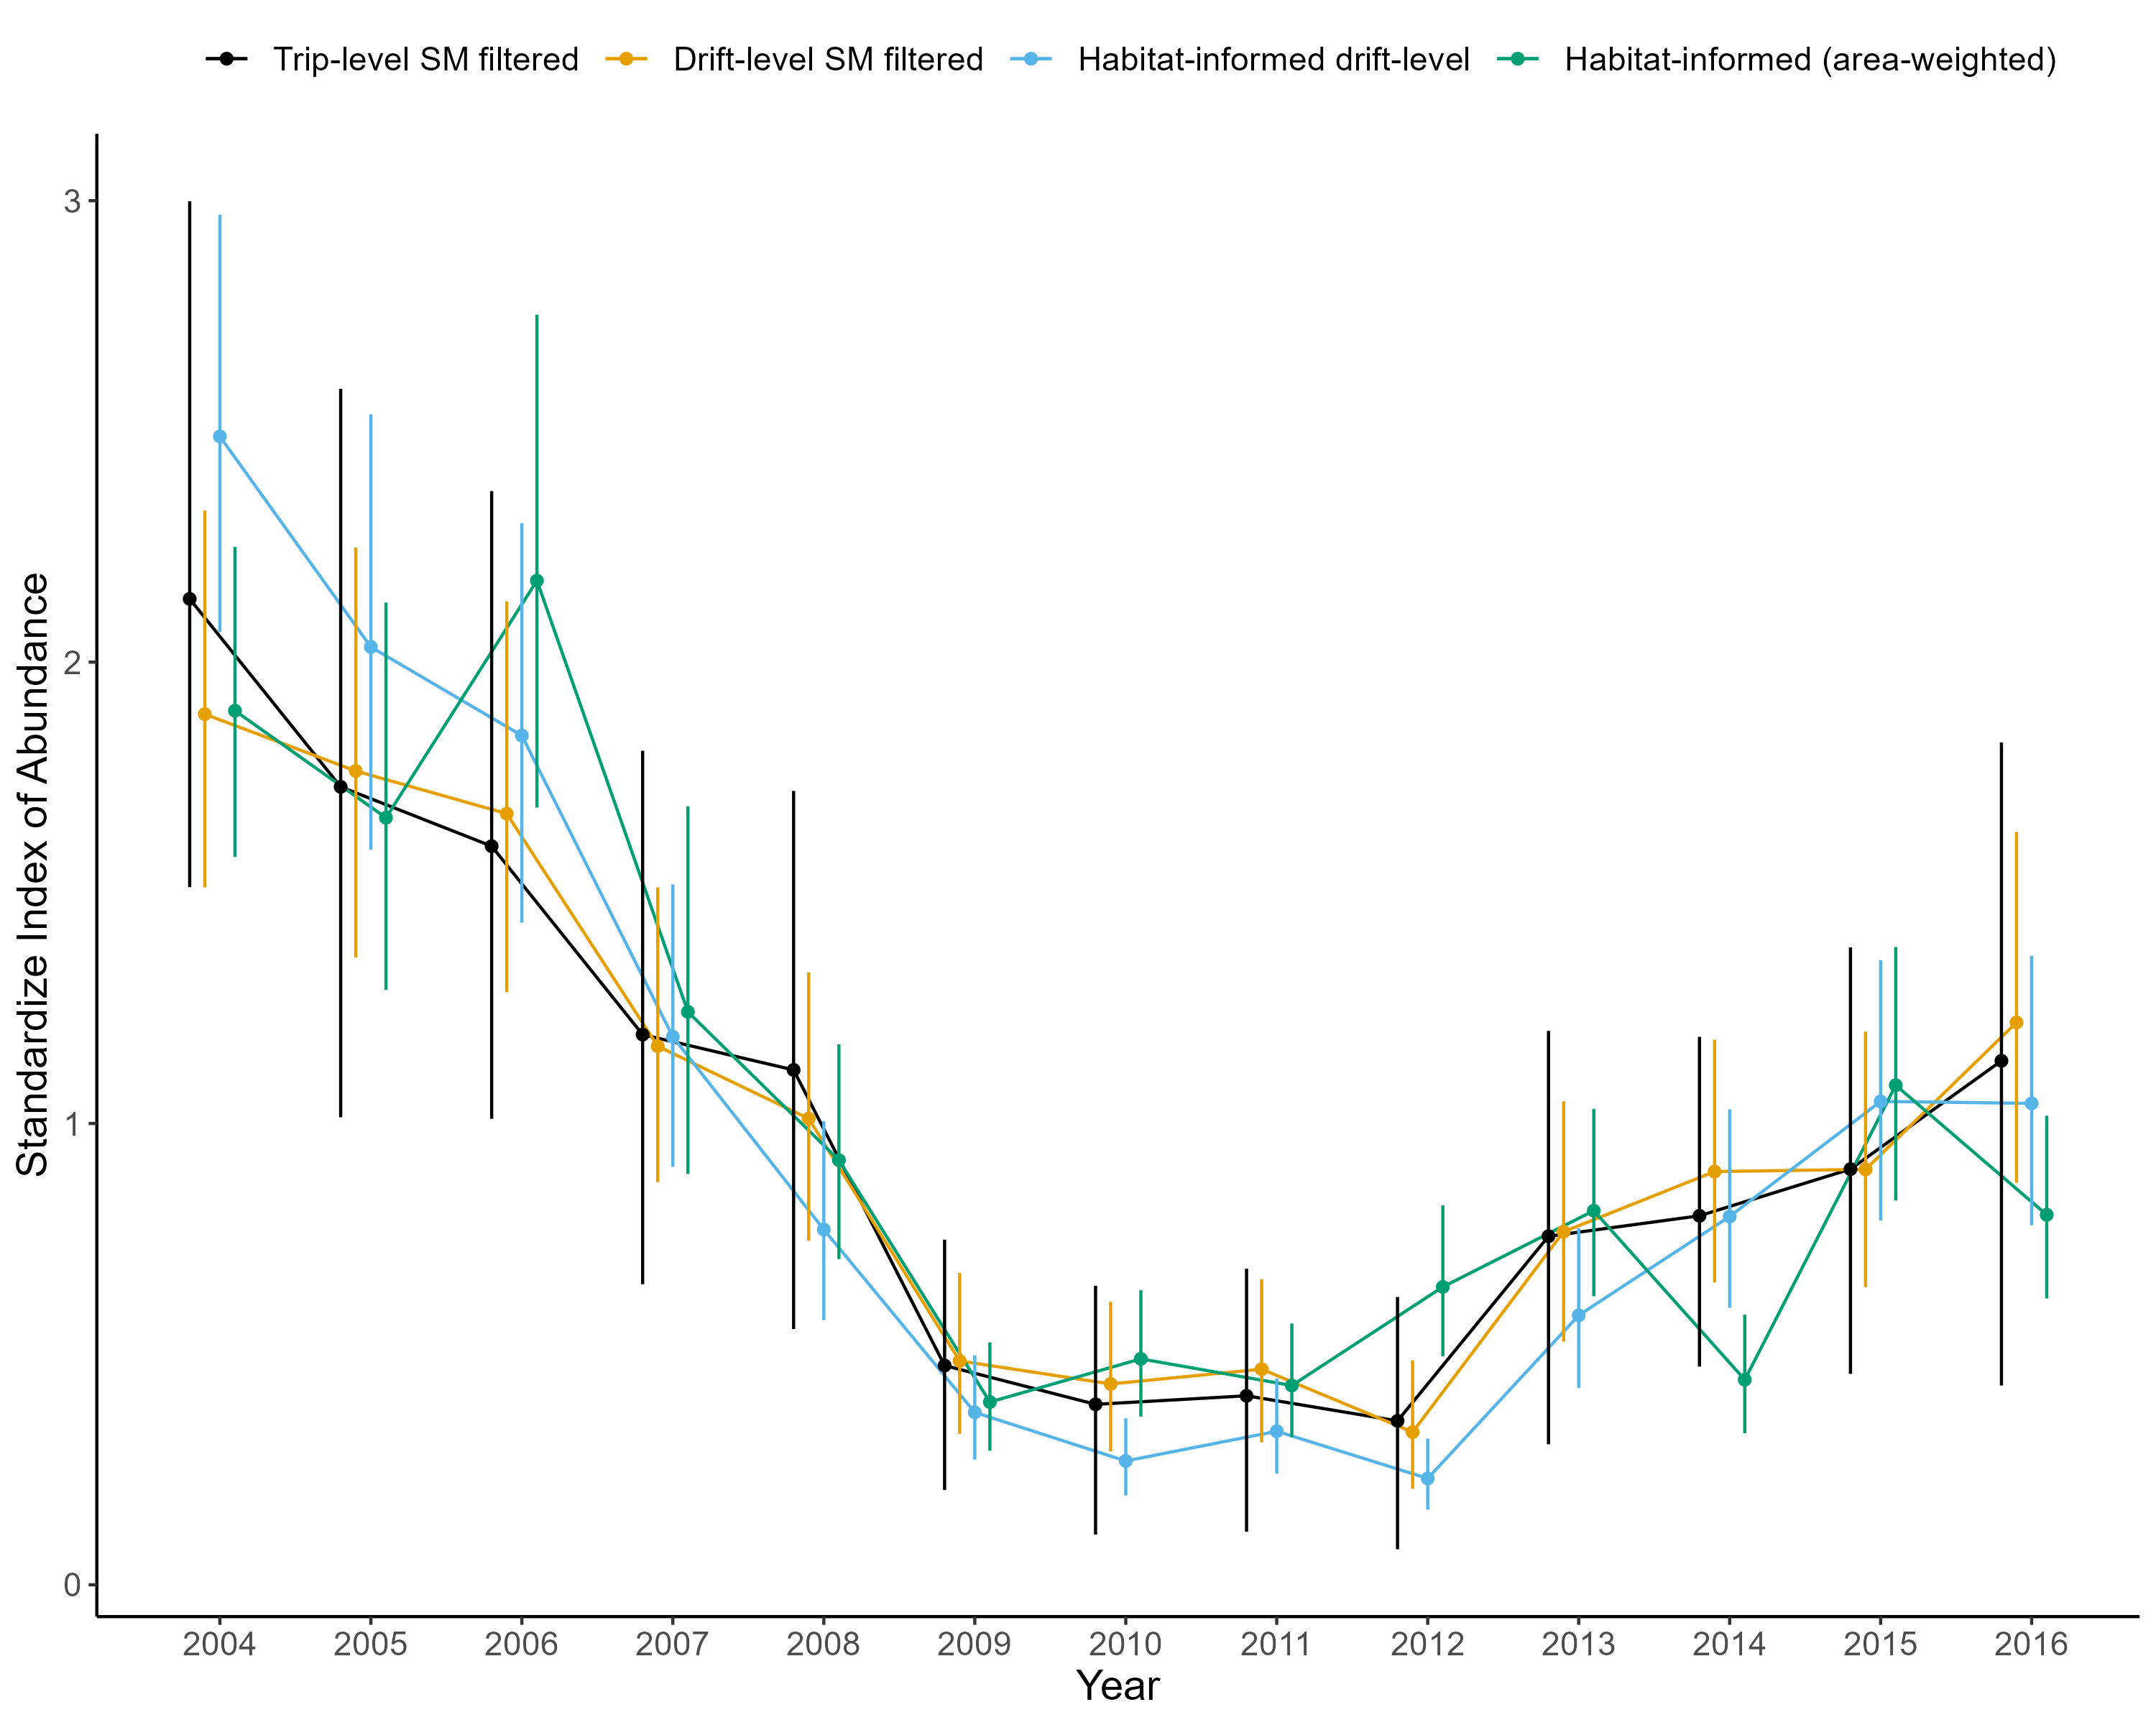
\includegraphics[width=3in,height=\textheight]{figures/blue_indices.png}

}

}

\subcaption{\label{fig-blue-indices}Blue rockfish}
\end{minipage}%
\newline
\begin{minipage}[t]{0.50\linewidth}

{\centering 

\raisebox{-\height}{

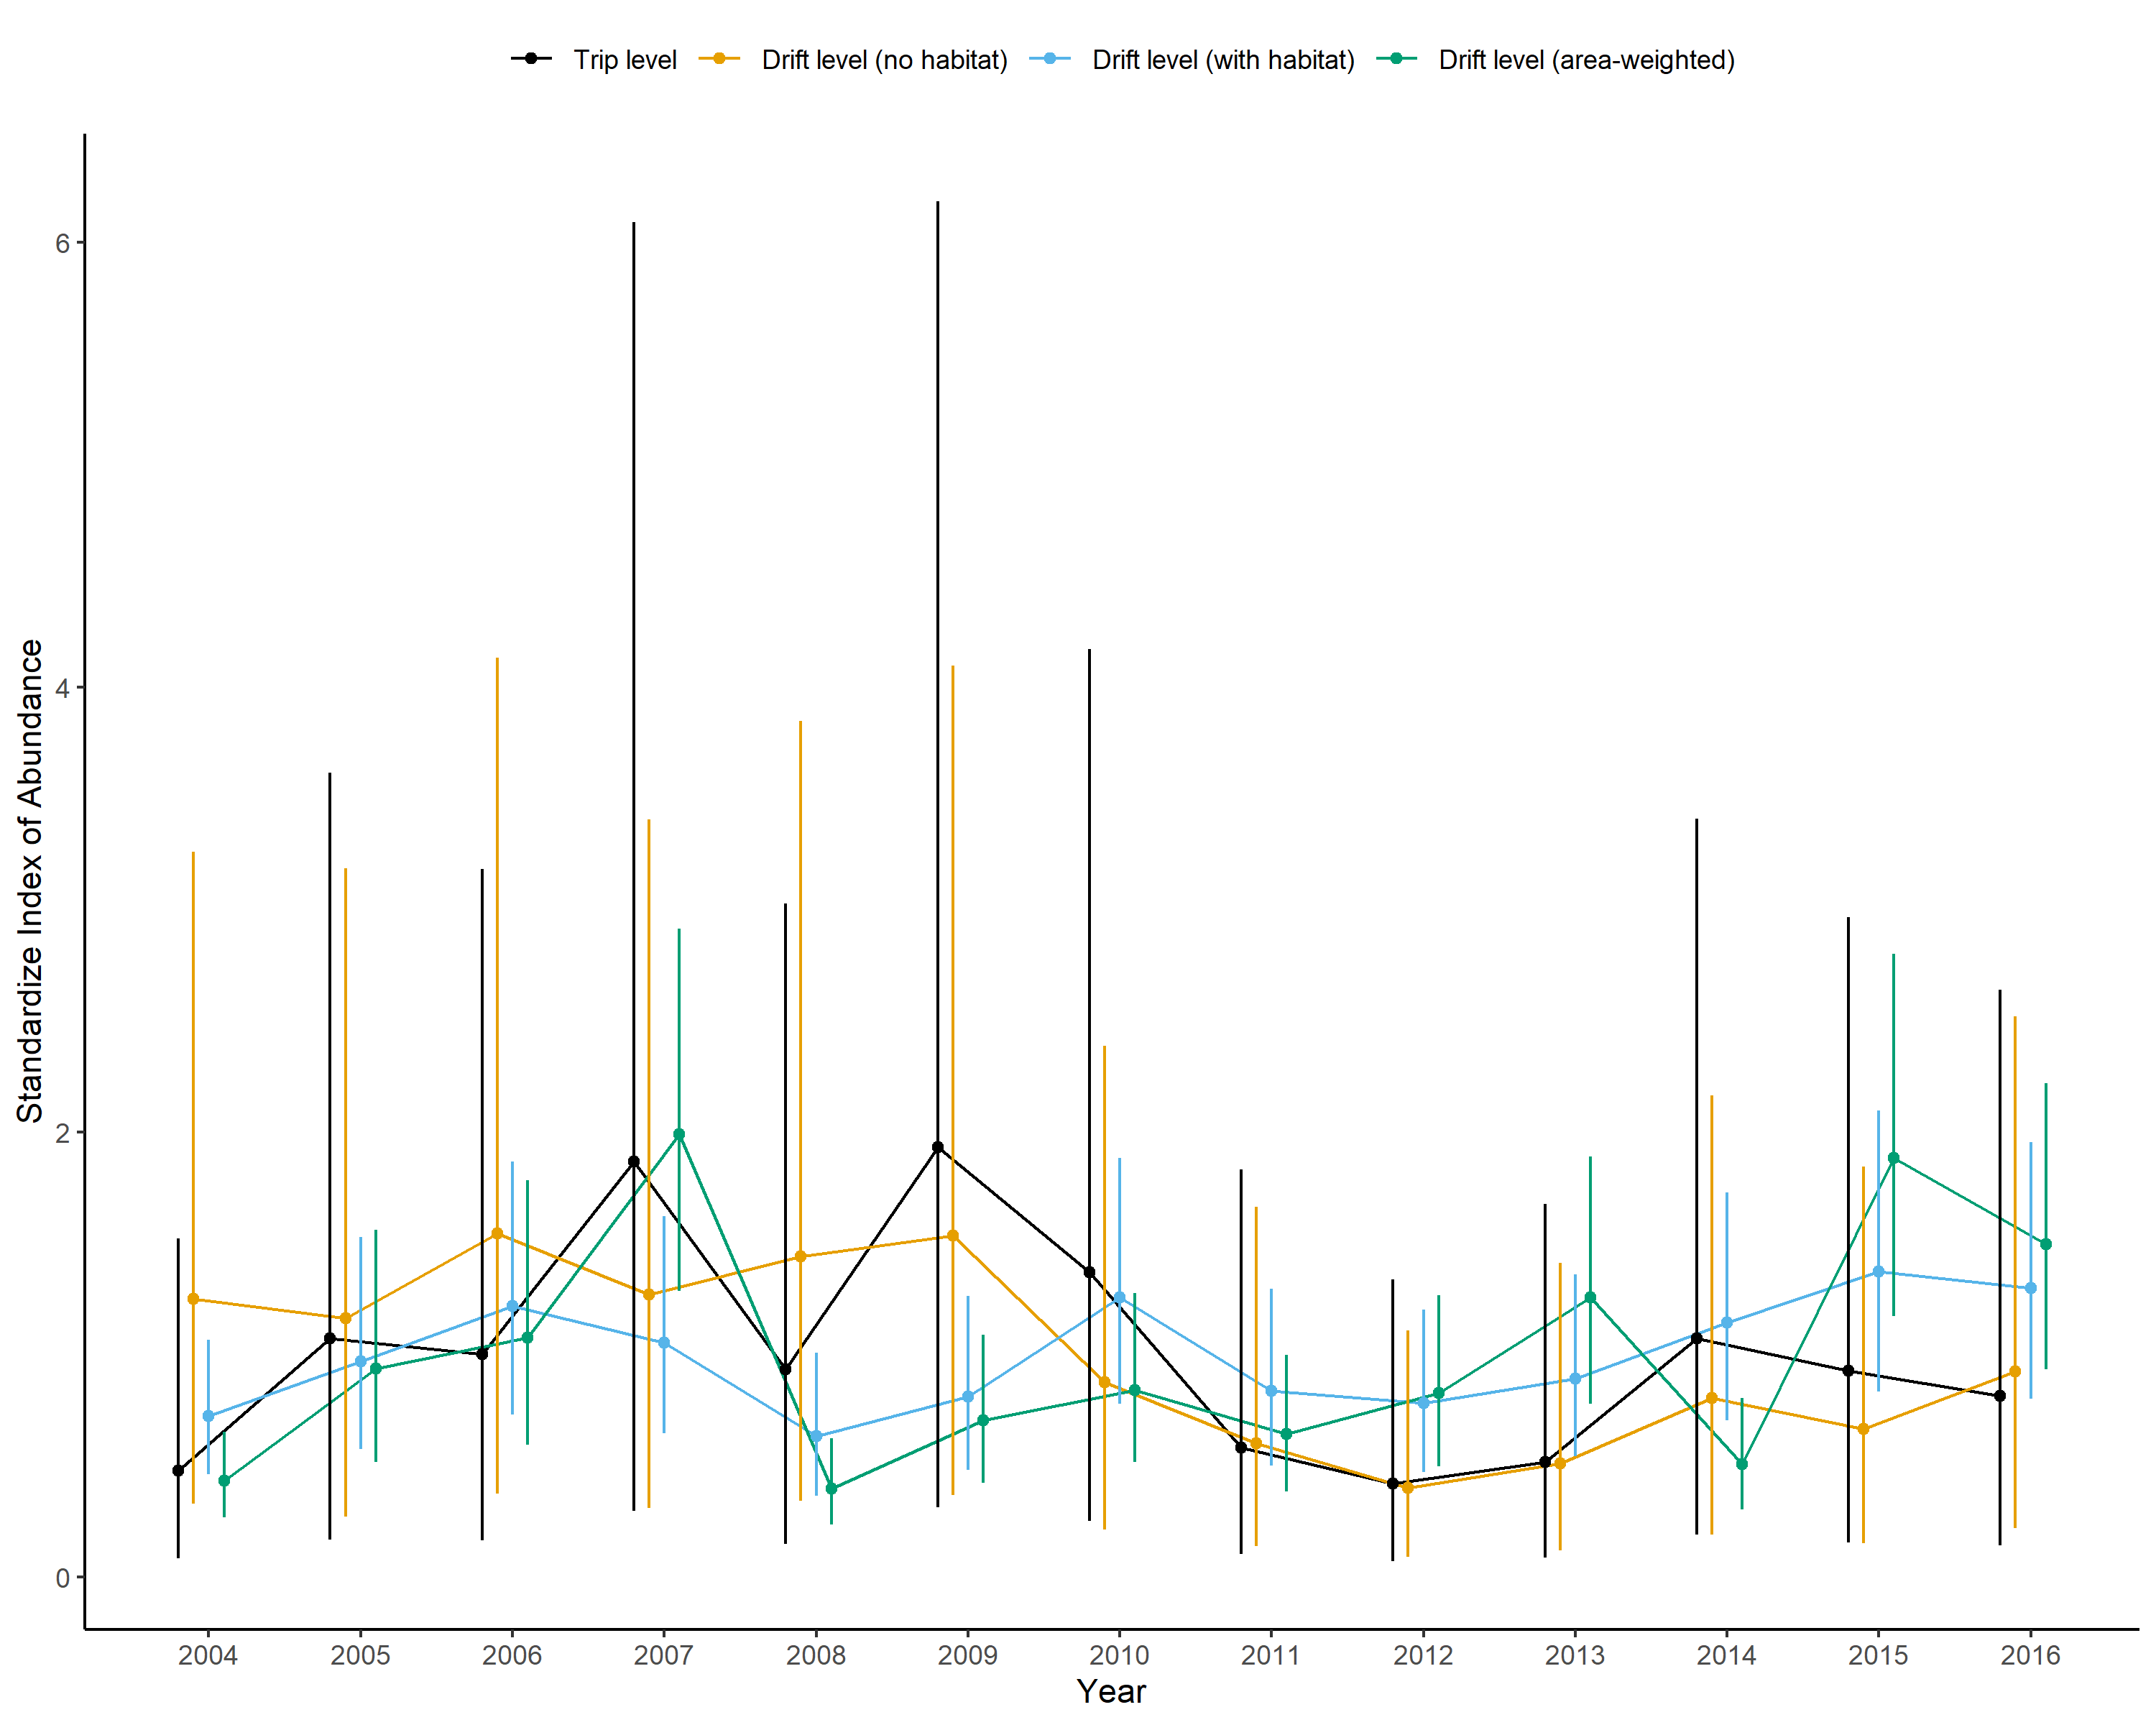
\includegraphics[width=3in,height=\textheight]{figures/brown_indices.png}

}

}

\subcaption{\label{fig-brown-indices}Brown rockfish}
\end{minipage}%
%
\begin{minipage}[t]{0.50\linewidth}

{\centering 

\raisebox{-\height}{

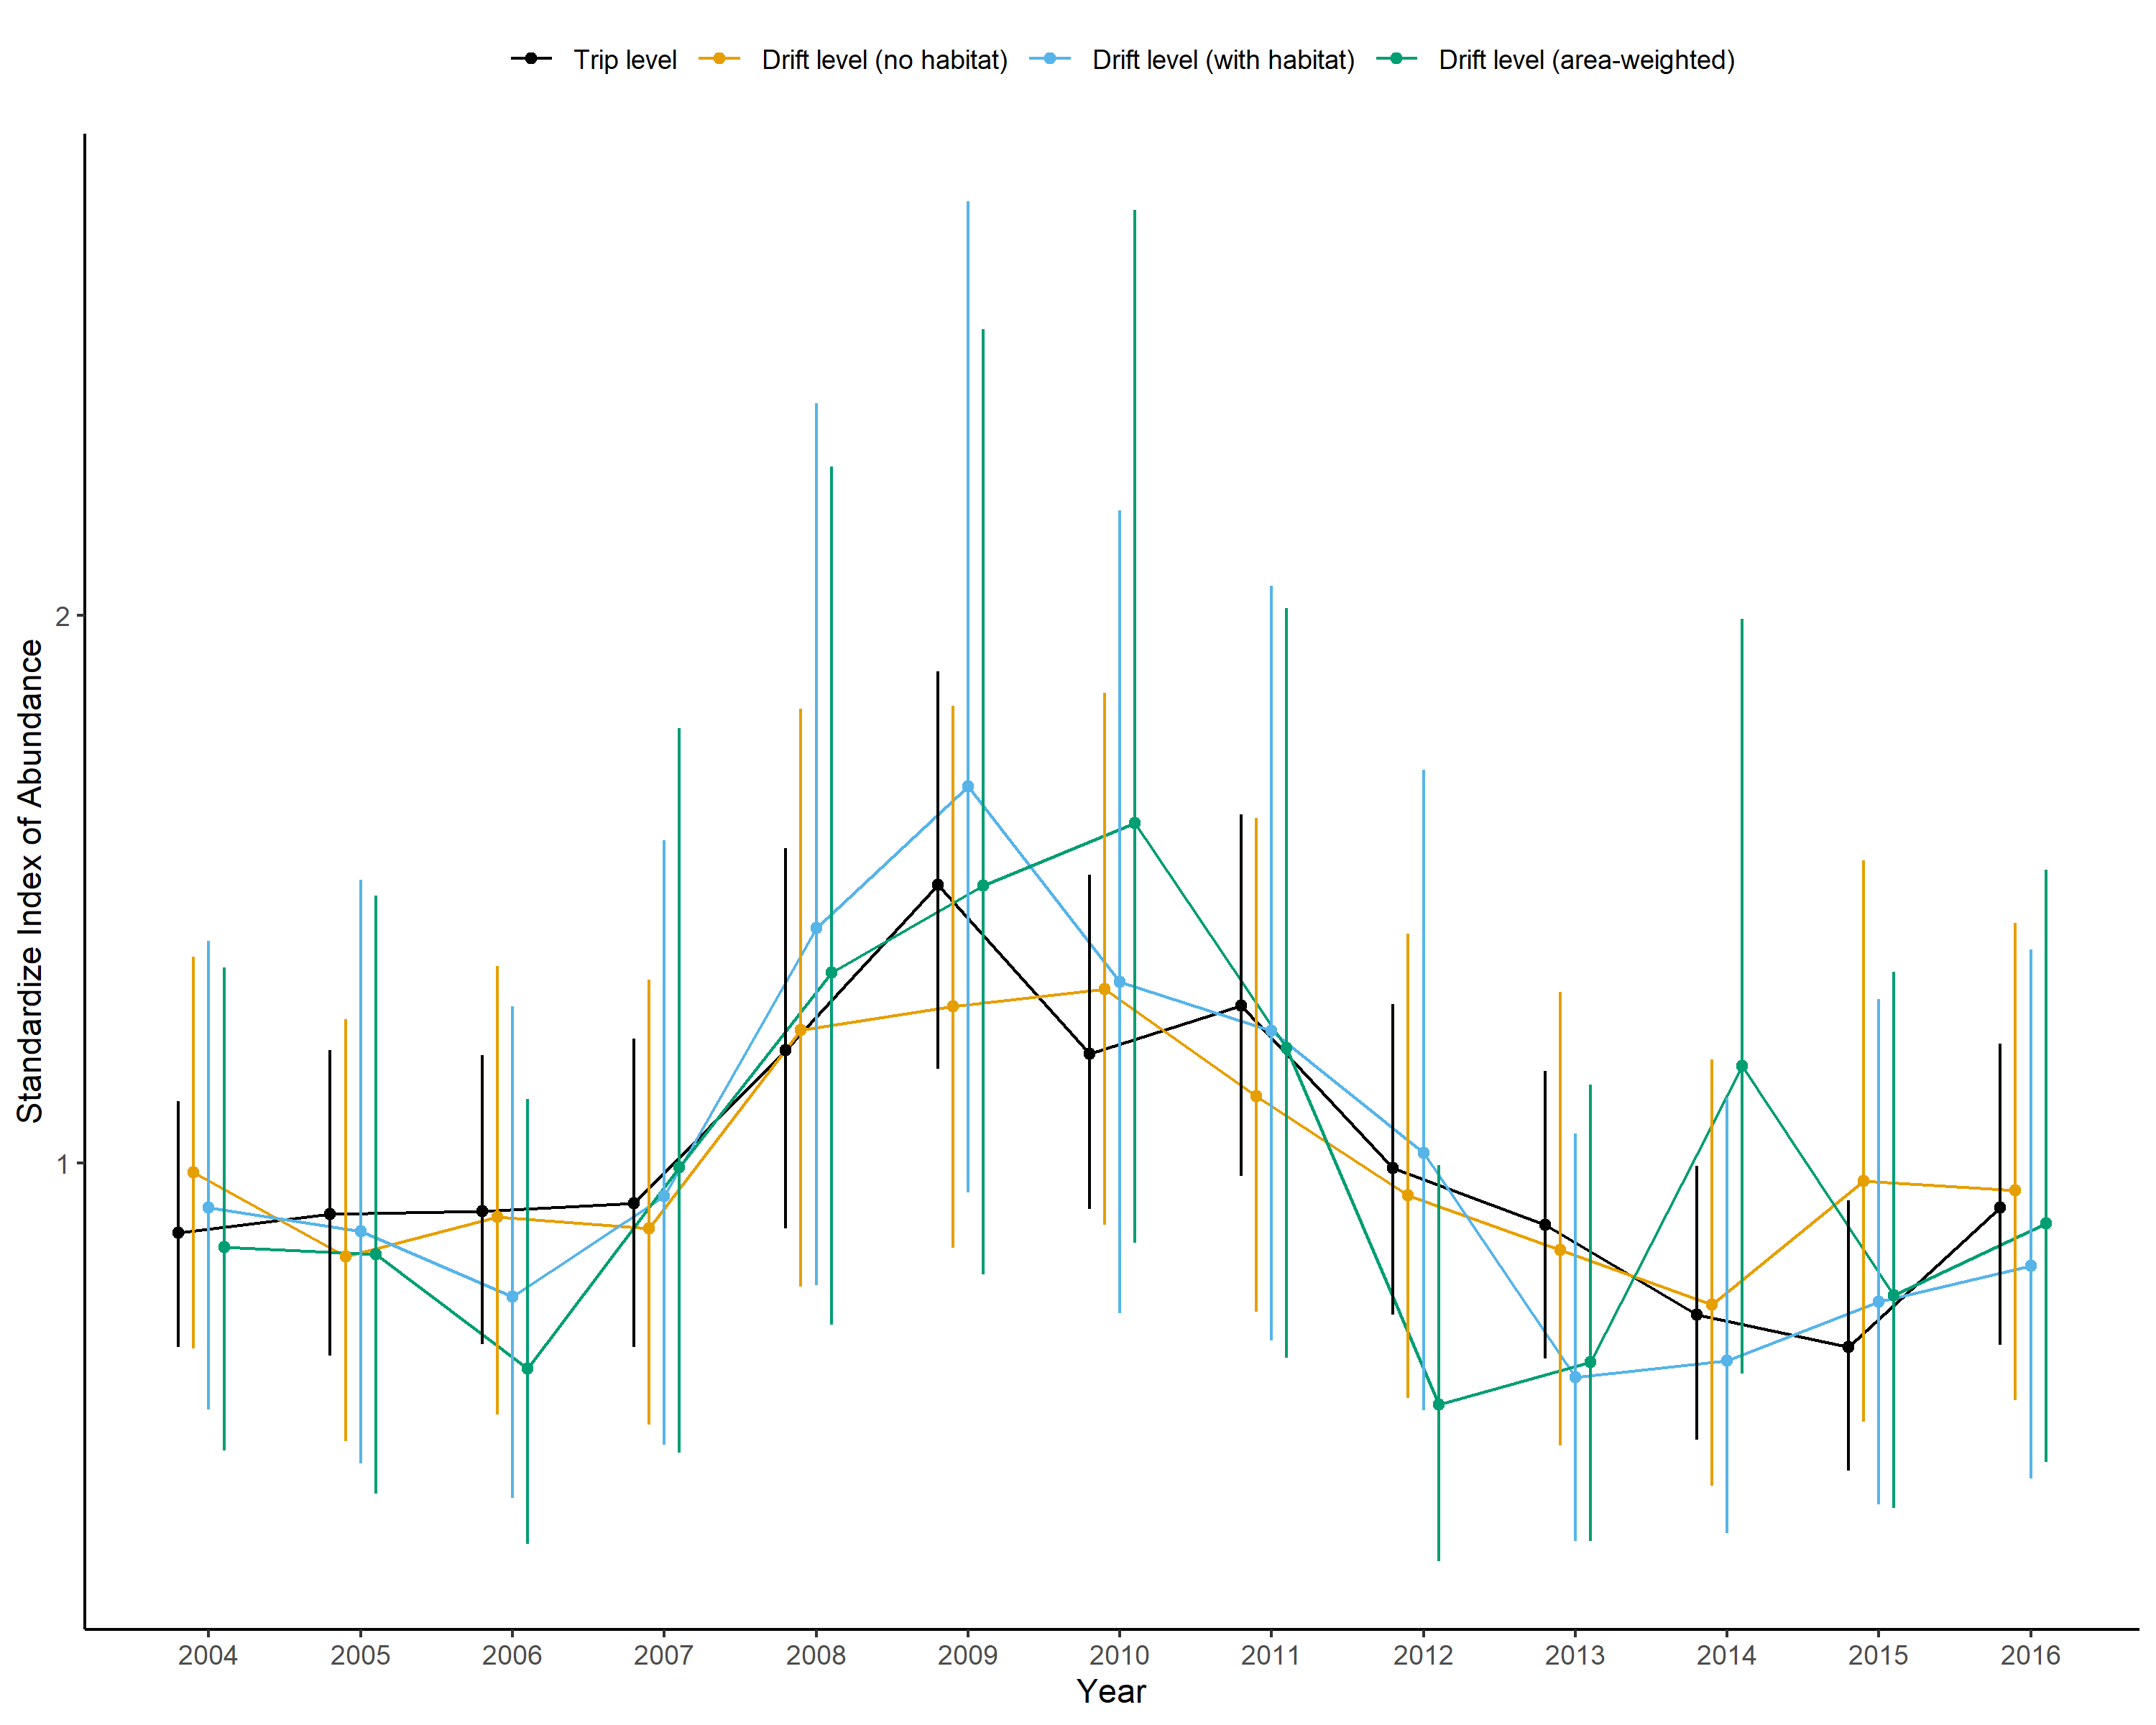
\includegraphics[width=3in,height=\textheight]{figures/china_indices.png}

}

}

\subcaption{\label{fig-china-indices}China rockfish}
\end{minipage}%
\newline
\begin{minipage}[t]{0.50\linewidth}

{\centering 

\raisebox{-\height}{

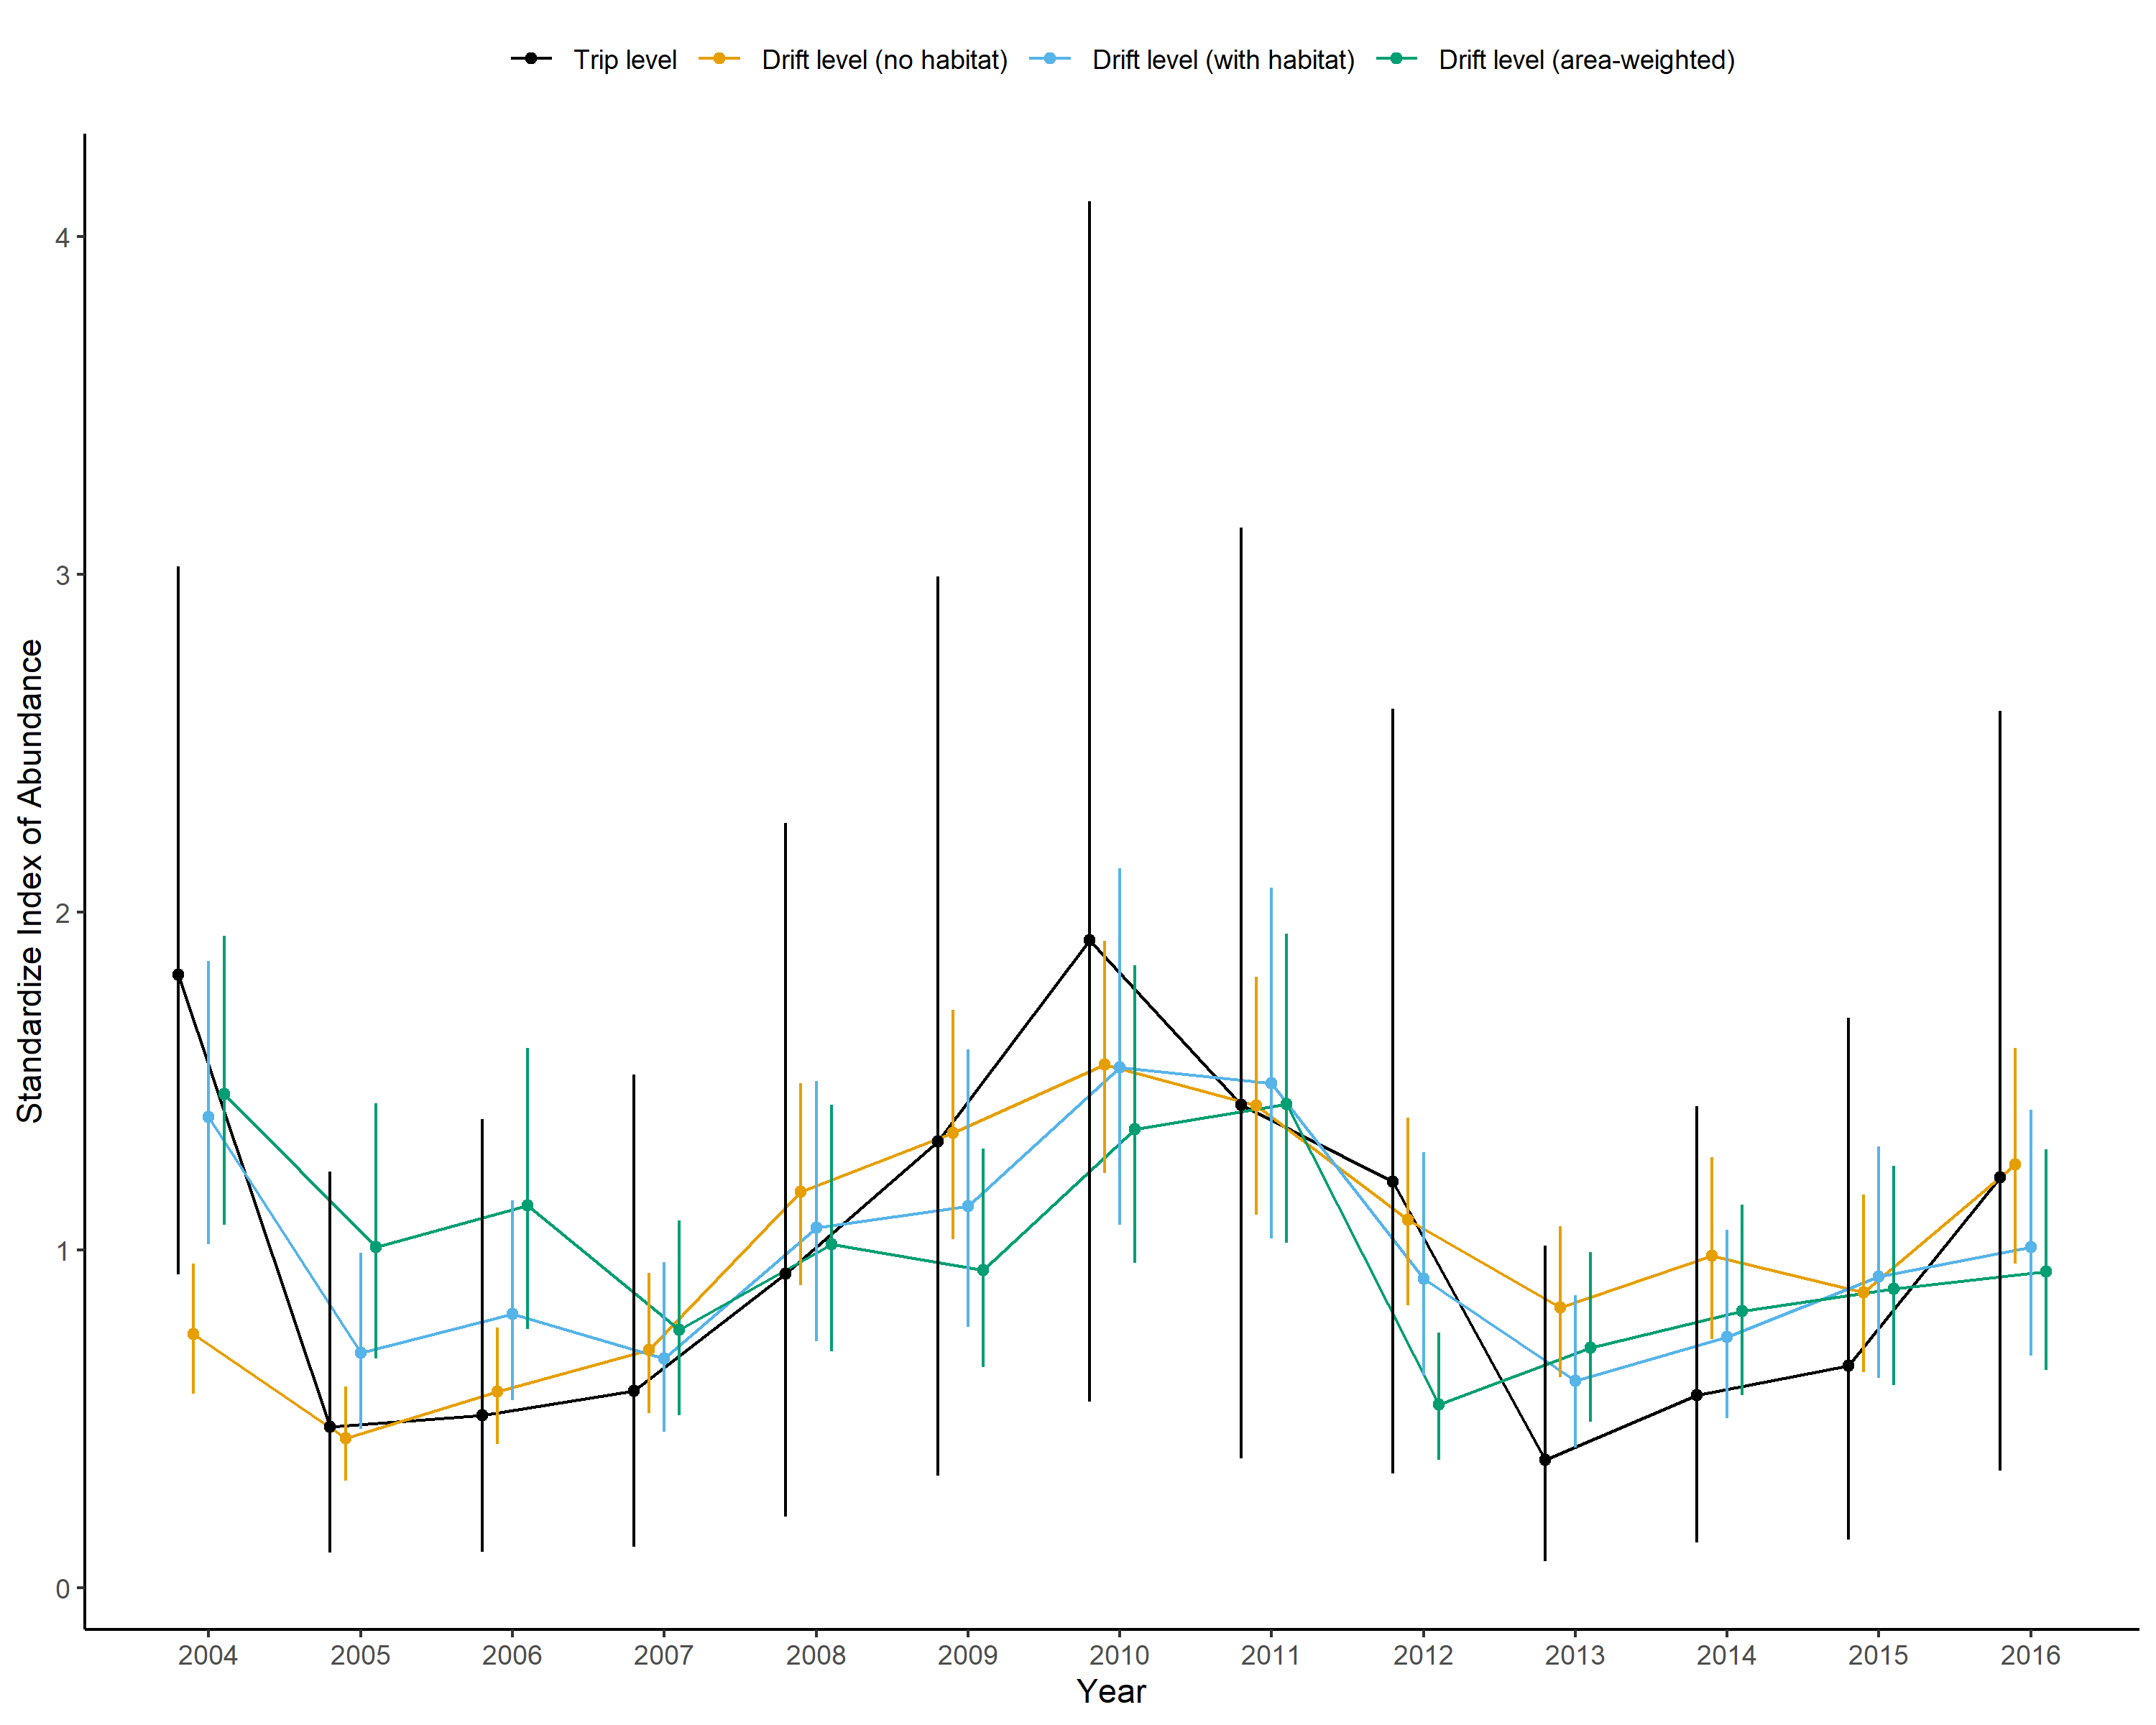
\includegraphics[width=3in,height=\textheight]{figures/gopher_indices.png}

}

}

\subcaption{\label{fig-gopher-indices}Gopher rockfish}
\end{minipage}%
%
\begin{minipage}[t]{0.50\linewidth}

{\centering 

\raisebox{-\height}{

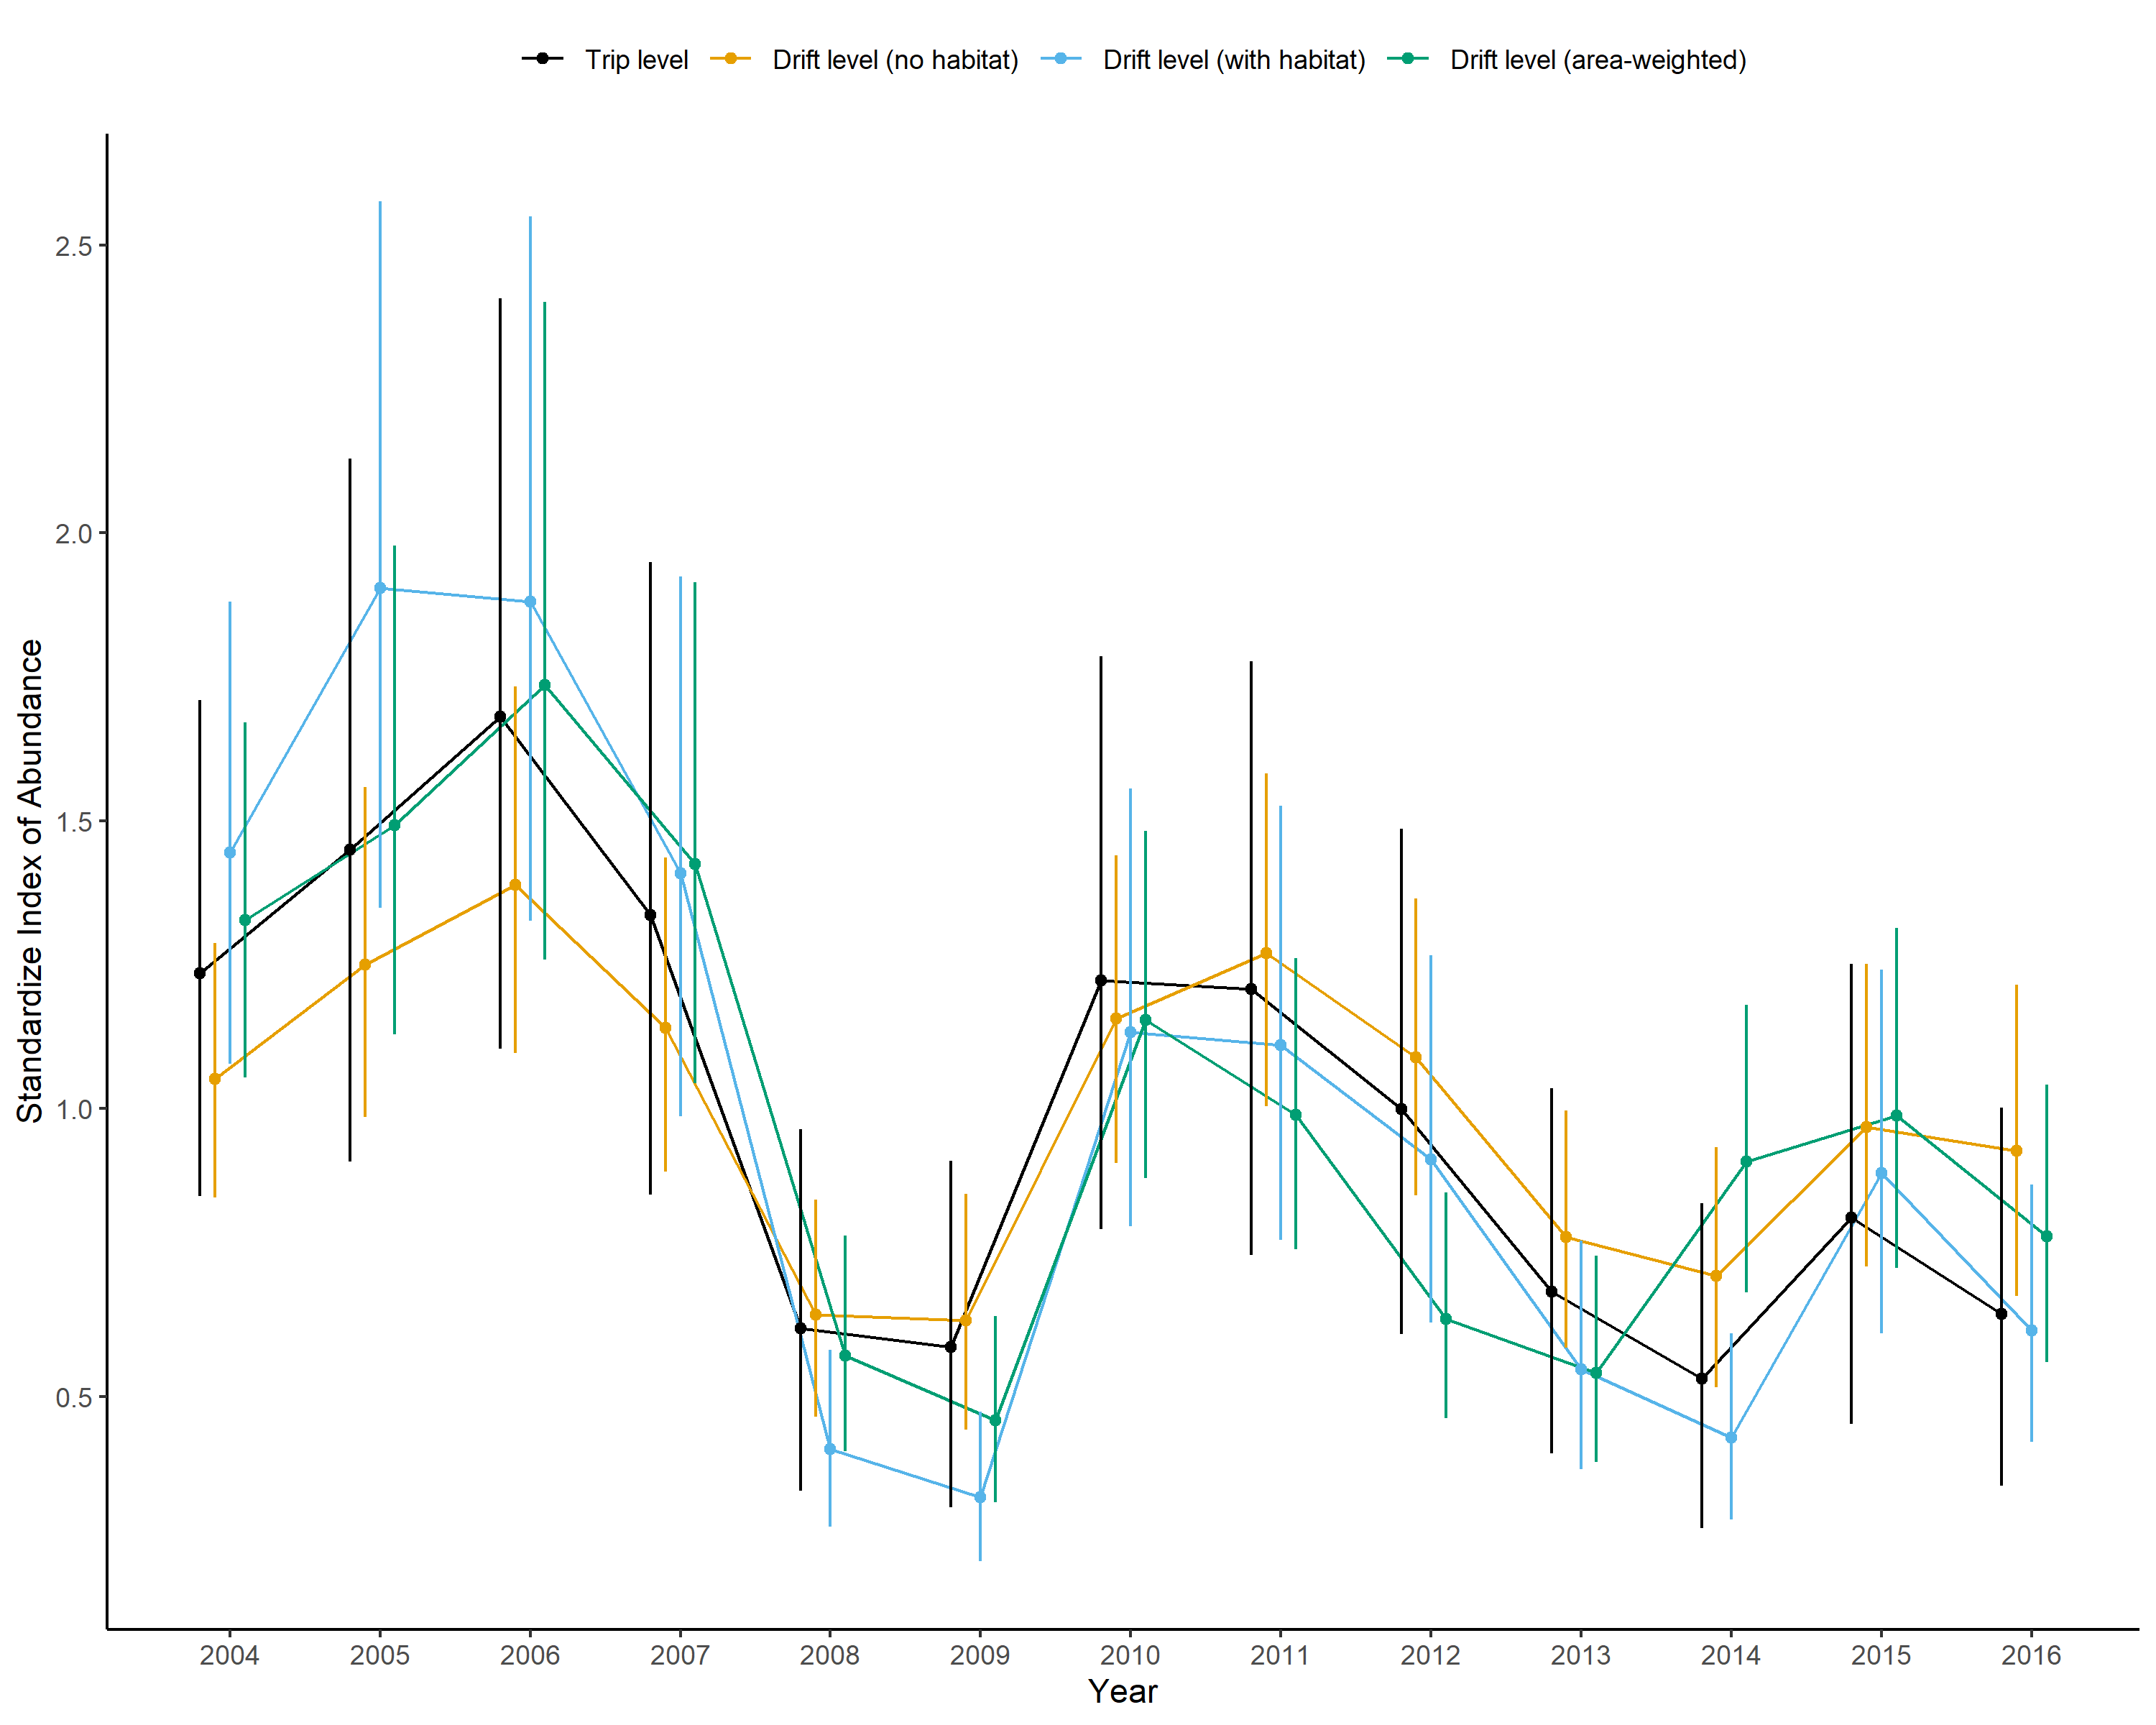
\includegraphics[width=3in,height=\textheight]{figures/vermilion_indices.png}

}

}

\subcaption{\label{fig-vermilion-indices}Vermilion rockfish}
\end{minipage}%

\caption{\label{fig-indices}Indices of abundance and 95\% confidence
intervals, each scaled to its mean, for the six species.}

\end{figure}

\FloatBarrier


  \bibliography{bibliography.bib}


\end{document}
